% UUM 523E Midterm Project report, Group 2
% Compile on Overleaf with the AIAA template class new-aiaa.cls
% (Overleaf: "Template for Submissions to AIAA Journals and Conferences").
% Tables in tables/*.tex hold the values of MT_Group2.mat and HW2_Group2.mat.
\documentclass[conf]{new-aiaa}
\usepackage[utf8]{inputenc}
\usepackage{graphicx}
\usepackage{amsmath}
\usepackage{booktabs}
\usepackage{multirow}
\usepackage{longtable,tabularx}
\setlength\LTleft{0pt}
% Table bodies are read with the primitive \@@input: the LaTeX \input is not
% expandable, so \bottomrule after it inside a tabular gives "Misplaced \noalign".
\makeatletter
\newcommand\tabinput[1]{\@@input #1 }
\AtBeginDocument{\@ifpackageloaded{hyperref}{\hypersetup{hidelinks}}{}}  % no link boxes
\makeatother

\title{F-16 Plant Model, Trim, Trimmed-Flight Simulation and Stability Analysis}

\author{Dilan Gelturan, Emirhan Oskay, Emircan S\"ur\"uc\"u and Berat Alku\footnote{Graduate students, Faculty of Aeronautics and Astronautics; UUM 523E Advanced Flight Dynamics, Group 2.}}
\affil{Istanbul Technical University, 34469 Maslak, Istanbul, Turkey}

\begin{document}

\maketitle

\begin{abstract}
A nonlinear six-degree-of-freedom F-16 model was built in Simulink from the NASA TP-1538 aerodynamic and engine data, trimmed with a constrained optimizer, and linearized numerically in body and wind axes. This report summarizes that work and uses it to study three trim conditions at Mach 0.6 and 10\,000 ft: wings-level flight with the center of gravity at $0.25\bar c$ (i), a $60^\circ$ banked level turn (ii), and wings-level flight with the center of gravity at $0.35\bar c$ (iii). Started from the trim points with fixed controls, the nonlinear model holds conditions i and ii for 60~s and one full turn with deviations below $10^{-2}$~m/s and $10^{-3}$~deg; in condition iii the states diverge slowly. Stability parameters and nondimensional derivatives are extracted from the wind-axis state matrices, with the inertia coupling of the roll and yaw rows removed and the thrust contribution to speed damping computed from the engine model. Condition iii is longitudinally statically unstable ($C_{m_\alpha}=+0.156$~rad$^{-1}$). With the leading-edge flap following its schedule in the linear model, the short period splits into two stable real roots and the phugoid becomes unstable with a time to double amplitude of 20.5~s, which explains the slow divergence seen in the simulation; with the flap fixed, an unstable root with a time to double amplitude of 0.88~s appears instead. In the turn, the trim angular rates add inertial terms to the state matrix and couple the phugoid and spiral modes, which shortens the phugoid period from 111~s to 57~s.
\end{abstract}

\section*{Nomenclature}

{\renewcommand\arraystretch{1.0}
\noindent\begin{longtable*}{@{}l @{\quad=\quad} l@{}}
$A$, $B$ & state and input matrices of the linear model \\
$a_{ij}$ & element $(i,j)$ of $A$ \\
$b$, $\bar c$, $S$ & wing span, mean aerodynamic chord, wing area, m, m, m$^2$ \\
$C_D$, $C_L$ & drag and lift coefficients \\
$C_l$, $C_m$, $C_n$ & rolling, pitching and yawing moment coefficients \\
$C_{D_u}$, $C_{m_u}$ & derivatives with respect to $\Delta V_T/U_1$ \\
$C_{(\cdot)_\alpha}$, $C_{(\cdot)_\beta}$ & derivatives with respect to $\alpha$ and $\beta$, rad$^{-1}$ \\
$C_{(\cdot)_q}$ & derivative with respect to $q\bar c/(2U_1)$, rad$^{-1}$ \\
$C_{(\cdot)_p}$, $C_{(\cdot)_r}$ & derivatives with respect to $pb/(2U_1)$ and $rb/(2U_1)$, rad$^{-1}$ \\
$h$ & altitude, m \\
$h_E$ & engine angular momentum, kg\,m$^2$/s \\
$I_{xx}$, $I_{yy}$, $I_{zz}$, $I_{xz}$ & moments and product of inertia (body axes), kg\,m$^2$ \\
$L_{(\cdot)}$, $M_{(\cdot)}$, $N_{(\cdot)}$ & rolling, pitching and yawing stability parameters \\
$m$ & aircraft mass, kg \\
$n_z$ & normal load factor \\
$p$, $q$, $r$ & body-axis roll, pitch and yaw rates, rad/s \\
$\bar q$ & dynamic pressure, Pa \\
$T$ & thrust, N \\
$t_{1/2}$, $t_2$ & times to half and to double amplitude, s \\
$U_1$ & total velocity at trim, m/s \\
$u$, $v$, $w$ & body-axis velocity components, m/s \\
$V_T$ & total velocity, m/s \\
$X_u$, $X_{T_u}$ & aerodynamic and thrust speed-damping parameters, s$^{-1}$ \\
$x_N$, $y_E$ & north and east positions, m \\
$x_{cg}$ & center-of-gravity position, fraction of $\bar c$ \\
$\alpha$, $\beta$ & angle of attack and sideslip angle, rad \\
$\gamma$ & flight-path angle, rad \\
$\delta_T$ & throttle setting, \% \\
$\delta_h$, $\delta_a$, $\delta_r$, $\delta_{lef}$ & stabilator, aileron, rudder and leading-edge-flap deflections, rad \\
$\zeta$, $\omega_n$ & damping ratio, natural frequency (rad/s) \\
$\lambda$ & eigenvalue, s$^{-1}$ \\
$\tau$ & time constant, s \\
$\phi$, $\theta$, $\psi$ & bank, pitch and heading angles, rad \\
$\boldsymbol\omega$ & body angular velocity vector $[p\ q\ r]^T$, rad/s \\
\multicolumn{2}{@{}l}{\emph{Subscripts}}\\
$1$ & trim (steady-state) value \\
$T$ & thrust contribution \\
\end{longtable*}}

\section{Introduction}

\lettrine{T}{his} report presents the course project of UUM 523E in three steps. In Homework 1, a nonlinear six-degree-of-freedom model of the F-16 was built in Simulink from the aerodynamic and engine data of NASA TP-1538~\cite{tp1538}, with the atmosphere and equations of motion of Stevens, Lewis and Johnson~\cite{slj}. In Homework 2, the model was trimmed at six flight conditions and linearized at three of them. The Midterm Project uses these results at three trim conditions, all at Mach 0.6 and 10\,000~ft with $\gamma=0$:
\begin{enumerate}
\item[i.] wings-level flight, $x_{cg}=0.25\bar c$;
\item[ii.] steady level turn with $\phi=60^\circ$ and $\beta=0$, $x_{cg}=0.25\bar c$;
\item[iii.] wings-level flight, $x_{cg}=0.35\bar c$.
\end{enumerate}
The nonlinear model is first flown from each trim point with the controls fixed (Sec.~IV). The stability parameters and nondimensional derivatives are then extracted from the wind-axis state matrices (Sec.~V), and the dynamic modes are computed from the full and decoupled matrices (Sec.~VI). Secs.~II and III summarize the plant model and the trim and linearization work on which these analyses rest.

All analyses are in MATLAB m-files that call the Homework 1 model (\texttt{F16\_6DOF.slx}, saved in R2023a), revised after the Homework 1 feedback as described in Sec.~II.C: \texttt{run\_HW1.m}, \texttt{run\_HW2.m} and \texttt{run\_MT.m}, the last of which writes the results file \texttt{MT\_Group2.mat}. All quantities are in SI units; angles are in rad unless stated otherwise.

\section{Plant Model}

\subsection{Structure}
The model (Fig.~\ref{fig:model}) consists of six subsystems built from basic Simulink blocks without the Aerospace Blockset: Atmosphere, Aerodynamics, Propulsion, Mass and Inertia, Actuators, and Equations of Motion. The leading-edge-flap (LEF) schedule is at the root level; the Aerodynamics, Propulsion and Mass and Inertia subsystems each output their own body-axis forces and moments, which are summed in the Equations of Motion. Mass, inertia and geometry are those of TP-1538 Table~I~\cite{tp1538} in SI units: $m=9295.4$~kg, $S=27.871$~m$^2$, $b=9.144$~m, $\bar c=3.4503$~m, $I_{xx}=12\,875$, $I_{yy}=75\,674$, $I_{zz}=85\,552$, $I_{xz}=1331.4$~kg\,m$^2$, and $h_E=216.93$~kg\,m$^2$/s.

\begin{figure}[hbt!]
\centering
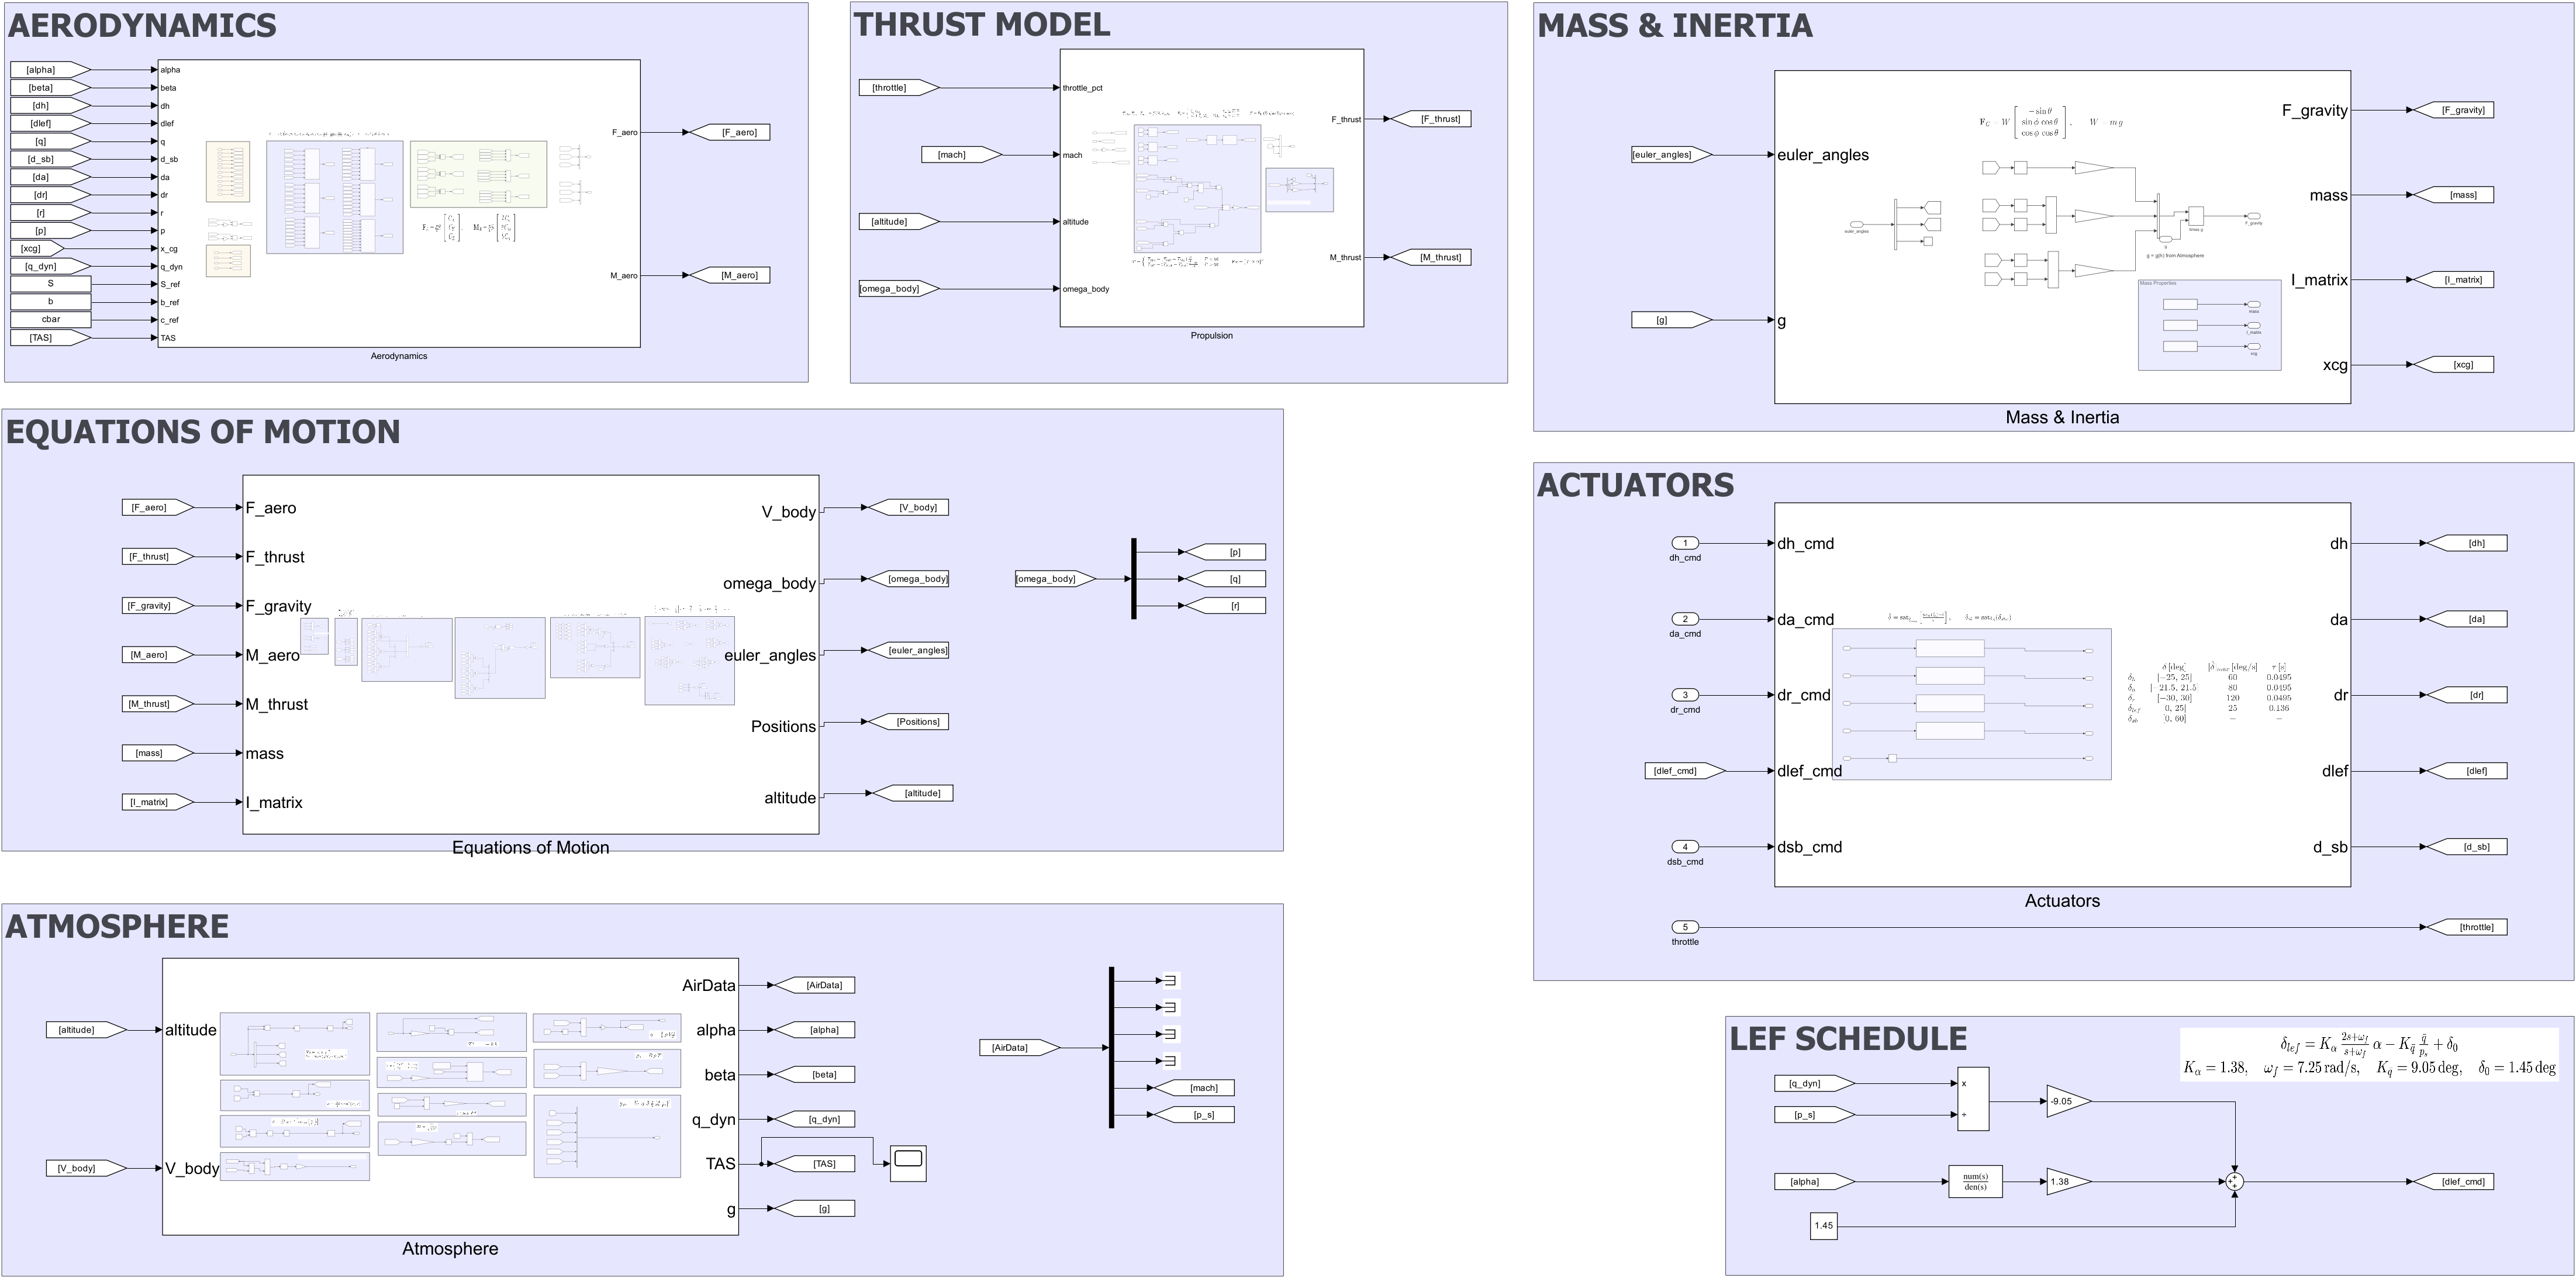
\includegraphics[width=\textwidth]{figures/MT_RootModel.png}
\caption{Root level of the F-16 Simulink model after the corrections of Sec.~II.C.}
\label{fig:model}
\end{figure}

\subsection{Subsystems}
\emph{Atmosphere.} The standard atmosphere of Ref.~\cite{slj}, Appendix A.6, gives the density, speed of sound, Mach number, static pressure and dynamic pressure; $\alpha=\operatorname{atan2}(w,u)$ and $\beta=\arcsin(v/V_T)$. The subsystem also outputs the gravitational acceleration $g=g_0[R_e/(R_e+h)]^2$, with $g_0=9.80665$~m/s$^2$ and $R_e=6.371\times10^6$~m.

\emph{Aerodynamics.} The six body-axis coefficients follow the TP-1538 build-up~\cite{tp1538}: base tables in $\alpha$, $\beta$ and $\delta_h$, LEF increments weighted by $(1-\delta_{lef}/25^\circ)$, control and speed-brake increments, and rate-damping terms in $q\bar c/(2V_T)$, $pb/(2V_T)$ and $rb/(2V_T)$, in 68 lookup tables. The data are referenced to $0.35\bar c$; the moments are transferred to the actual center of gravity by $C_m \leftarrow C_m + C_Z(0.35-x_{cg})$ and $C_n \leftarrow C_n - C_Y(0.35-x_{cg})\bar c/b$~\cite{slj}.

\emph{Propulsion.} The throttle gearing maps $\delta_T$ to a power command (77\,\% gives military power); a first-order lag with power-dependent time constant gives the power level $P_3$, and the thrust is interpolated between the idle, military and maximum tables of Mach number and altitude~\cite{tp1538}. The thrust $\mathbf F_T=[T\ 0\ 0]^T$ acts along the body $x$ axis through the center of gravity. The subsystem also outputs the engine gyroscopic moment $\mathbf M_T=-\boldsymbol\omega\times\mathbf h_E=[0\ \ {-r}h_E\ \ qh_E]^T$, with $\mathbf h_E=[h_E\ 0\ 0]^T$.

\emph{Mass and inertia.} The subsystem computes the gravity force $\mathbf F_G=mg[-\sin\theta\ \ \sin\phi\cos\theta\ \ \cos\phi\cos\theta]^T$ with $g$ from the Atmosphere, and outputs the mass, the inertia matrix and the center-of-gravity position, which the Aerodynamics subsystem and the equations of motion use.

\emph{Actuators.} The stabilator, aileron, rudder and LEF actuators are separate subsystems, each a first-order lag with position and rate limits (time constants 0.0495~s and 0.136~s for the LEF)~\cite{tp1538}.

\emph{Equations of motion.} For a rigid aircraft of constant mass over a flat, nonrotating Earth~\cite{slj},
\begin{equation}
m(\dot{\mathbf v}+\boldsymbol\omega\times\mathbf v)=\mathbf F_A+\mathbf F_T+\mathbf F_G, \qquad
\mathbf I\dot{\boldsymbol\omega}+\boldsymbol\omega\times\mathbf I\boldsymbol\omega=\mathbf M_A+\mathbf M_T,
\label{eq:eom}
\end{equation}
together with the Euler-angle kinematics and the north--east--down position. The forces and moments are summed inside this subsystem.

\emph{LEF schedule.} $\delta_{lef}=1.38\,\dfrac{2s+7.25}{s+7.25}\,\alpha-9.05\,\bar q/p_s+1.45$ (degrees), limited to $0$--$25^\circ$~\cite{slj}.

\subsection{Verification and corrections}
The Aerodynamics and Propulsion blocks were run alone in test models and agreed with independent reference calculations in all ten coefficient cases and all five thrust cases of Homework 1. At the reference center of gravity the aircraft is statically unstable in pitch at small angles of attack, with a static margin of about $-4\,\%\,\bar c$, the relaxed-stability configuration studied in TP-1538~\cite{tp1538}.

\emph{Corrections.} The course data give $C_{l_p}(\alpha=55^\circ)=-1200$; it is replaced by the TP-1538 value $-0.12$ when the data are loaded. This correction was already made in Homework 1 and does not affect the present conditions ($\alpha<11^\circ$). After the Homework 1 feedback, the model was revised in five points:
\begin{enumerate}
\item each actuator is a separate subsystem (they were in one block);
\item the gravitational acceleration varies with altitude and is an output of the Atmosphere subsystem (it was the constant $g_0$);
\item the mass, the inertia matrix and the center-of-gravity position are outputs of the Mass and Inertia subsystem (they were workspace constants used directly in the equations of motion and at the root level);
\item the engine gyroscopic moment is computed in the Propulsion subsystem (it was in the equations of motion);
\item the forces and moments are summed in the Equations of Motion subsystem (they were summed at the root level).
\end{enumerate}
The other items of the feedback (LEF schedule and actuator, gravity force, engine dynamics) were already in the model. With $g$ held constant, the revised model reproduces the state derivatives of the Homework 1 model to $6\times10^{-11}$ at arbitrary states, so items 1 and 3--5 change no result. The only physical change is $g(h)$, which is 0.1\,\% smaller than $g_0$ at 10\,000~ft.

\section{Trim and Linearization}

\subsection{Trim}
The trim problem is solved with \texttt{fmincon} (SQP). The unknowns are $\alpha$, $\beta$, $\phi$, $\theta$, the turn rate $\dot\psi$ and the four controls; $V_T$ and $h$ follow from the specified Mach number and altitude. In a steady turn the body rates are $p=-\dot\psi\sin\theta$, $q=\dot\psi\sin\phi\cos\theta$ and $r=\dot\psi\cos\phi\cos\theta$, so that $\dot\phi=\dot\theta=0$. The cost function~\cite{slj}
\begin{equation}
J=\dot V_T^2+100(\dot\alpha^2+\dot\beta^2)+10(\dot p^2+\dot q^2+\dot r^2)
\end{equation}
is minimized subject to the flight-path-angle constraint and, where specified, the load-factor constraint. As in Lecture 4, the load factor of case 5 is $n_z=1/\cos\mu$, with the wind-axis bank angle $\tan\mu=\cos\theta\sin\phi/(\sin\alpha\sin\theta+\cos\alpha\cos\theta\cos\phi)$, so the constraint is $f_{NLF}=n_z-1/\cos\mu=0$. The LEF is set by the steady-state schedule at every evaluation. Table~\ref{tab:trim} lists the six trim points; $J<10^{-10}$ in all cases, and the model derivatives at trim, including the actuator, engine and LEF-filter states, vanish to $2\times10^{-4}$~m/s$^2$ and $10^{-6}$~rad/s$^2$. Conditions i, ii and iii of this report are cases 1, 4 and 6.

\begin{table}[hbt!]
\caption{\label{tab:trim} Trim results of Homework 2, recomputed with the revised model (angles in deg, $\dot\psi$ in rad/s)}
\centering
\small
\setlength\tabcolsep{3.5pt}
\begin{tabular}{clccccccccccc}
\toprule
Case & $M$, $h$ [ft], spec. & $x_{cg}$ & $V_T$ [m/s] & $\alpha$ & $\theta$ & $\phi$ & $\dot\psi$ & $\delta_T$ [\%] & $\delta_h$ & $\delta_a$ & $\delta_r$ & $\delta_{lef}$ \\
\midrule
\tabinput{tables/trim.tex}
\bottomrule
\end{tabular}
\end{table}

\subsection{Linearization}
The model is linearized by central differences about each trim point, perturbing one state or input at a time by $10^{-3}$ (in m/s, rad, rad/s and \%, as in Lecture~5); the derivatives are read from the Simulink model through its model API. The wind-axis model used in this report has
\begin{equation}
\Delta\mathbf x=[\Delta V_T\ \Delta\alpha\ \Delta q\ \Delta\theta\ \Delta\beta\ \Delta p\ \Delta r\ \Delta\phi]^T,\qquad
\Delta\mathbf u=[\Delta\delta_T\ \Delta\delta_h\ \Delta\delta_a\ \Delta\delta_r]^T,
\end{equation}
with $A=\begin{bmatrix}A_{11}&A_{21}\\A_{12}&A_{22}\end{bmatrix}$ partitioned into the longitudinal block $A_{11}$, the lateral-directional block $A_{22}$ and the coupling blocks. The actuator and engine states are not part of the 8-state model. The LEF follows its schedule: at every perturbed state, $\delta_{lef}$ is recomputed from the perturbed $\alpha$ and $\bar q/p_s\propto V_T^2$ (the filter $(2s+7.25)/(s+7.25)$ has unit steady-state gain). Only Problem 2 (Sec.~V) uses a second model with $\delta_{lef}$ held at its trim value. The schedule changes three elements: through $\partial\delta_{lef}/\partial\alpha=1.38$, the flap adds a nose-down moment and drag as $\alpha$ grows, so $a_{32}$ decreases by 1.93, 2.16 and 2.42~s$^{-2}$ in i, ii and iii, $a_{12}$ decreases by 3.0 and 3.3~m\,s$^{-2}$ in i and iii (it is almost unchanged in ii), and $a_{22}$ increases by 0.06~s$^{-1}$.

\emph{Comparison of the three conditions.} Table~\ref{tab:alin} lists the main elements of $A_W$ and $B_W$ that change between the conditions. The speed-damping and rate elements that change in the turn ($a_{11}$, $a_{13}$, $a_{67}$) are discussed with the stability parameters in Sec.~V.
\begin{itemize}
\item $a_{32}$ (pitch stiffness, $M_\alpha$ with the LEF contribution): moving the center of gravity aft from $0.25\bar c$ to $0.35\bar c$ removes the moment transfer $C_Z(0.35-x_{cg})$, i.e., the stabilizing arm of the lift ahead of the center of gravity, and $a_{32}$ changes sign. The aircraft is statically unstable in pitch in iii, and the LEF schedule only reduces the instability. In the turn, $a_{32}$ is 9\,\% larger in magnitude because $\alpha_1$ is higher and $\bar q$ is the same.
\item $a_{33}$ (pitch damping): the tail is the main source of damping, and its arm about the center of gravity is shorter in iii, so the damping falls by 36\,\%.
\item $b_{32}$ (stabilator power): for the same reason the stabilator moment arm, and thus its pitch control power, is 8\,\% smaller in iii.
\item $a_{12}$ (speed change with $\alpha$): in wings-level flight, raising $\alpha$ at constant $\theta$ tilts the flight path down, and gravity accelerates the aircraft ($+g\cos\theta_1=9.8$~m\,s$^{-2}$) more than the extra drag decelerates it, so $a_{12}>0$. In the $60^\circ$ turn only $g\cos\phi_1$ of gravity acts in the plane of $\alpha$, and the drag gradient is larger because $C_{L_1}$ is twice as large (induced drag $\propto C_L^2$), so $a_{12}$ becomes strongly negative.
\item $a_{15}$, $a_{18}$, $a_{43}$, $a_{47}$ (coupling): in straight flight the coupling blocks are zero. In the turn, sideslip and bank change the component of gravity along the flight path ($a_{15}\approx g\cos\theta_1\sin\phi_1$), and the pitch kinematics $\dot\theta=q\cos\phi-r\sin\phi$ link $\theta$ to both $q$ and $r$. The longitudinal and lateral-directional motions are therefore coupled (Sec.~VI).
\item $a_{65}$ (dihedral effect): $L_\beta$ is 33\,\% larger in the turn because the dihedral effect of the swept wing grows with $\alpha$ and $C_L$.
\item $a_{75}$ (directional stiffness): the vertical tail arm is shorter with the aft center of gravity, so $N_\beta$ is 18\,\% smaller in iii.
\item $a_{76}$: in the turn, the trim rates add the inertial term $\partial[\boldsymbol\omega\times\mathbf I\boldsymbol\omega]_z/\partial p=(I_{yy}-I_{xx})q_1$ to the yaw equation, so $\partial\dot r/\partial p$ is eight times its straight-flight value.
\end{itemize}
Physically, the forward-center-of-gravity conditions are stiff and well damped in pitch, the aft center of gravity gives a pitch-unstable airframe with less control power, and the turn adds kinematic and inertial coupling between the two motions while leaving the fast dynamics nearly unchanged.

\begin{table}[hbt!]
\caption{\label{tab:alin} Elements of $A_W$ and $B_W$ (scheduled LEF) that change between the conditions}
\centering
\begin{tabular}{llccc}
\toprule
Element & Unit & i & ii & iii \\
\midrule
\tabinput{tables/alin.tex}
\bottomrule
\end{tabular}
\end{table}

Figure~\ref{fig:linnl} compares the linear and nonlinear responses in condition iii. With the scheduled LEF in the linear model, the two agree in all channels over 10~s. With a $1^\circ$ doublet the nonlinear model departs: the trim deflection is only $\delta_{lef}=1.14^\circ$, so a nose-down change of $0.8^\circ$ in $\alpha$ drives the flap to its $0^\circ$ limit, its stabilizing feedback is lost, and the fast pitch divergence of the fixed-flap airframe appears.

\begin{figure}[hbt!]
\centering
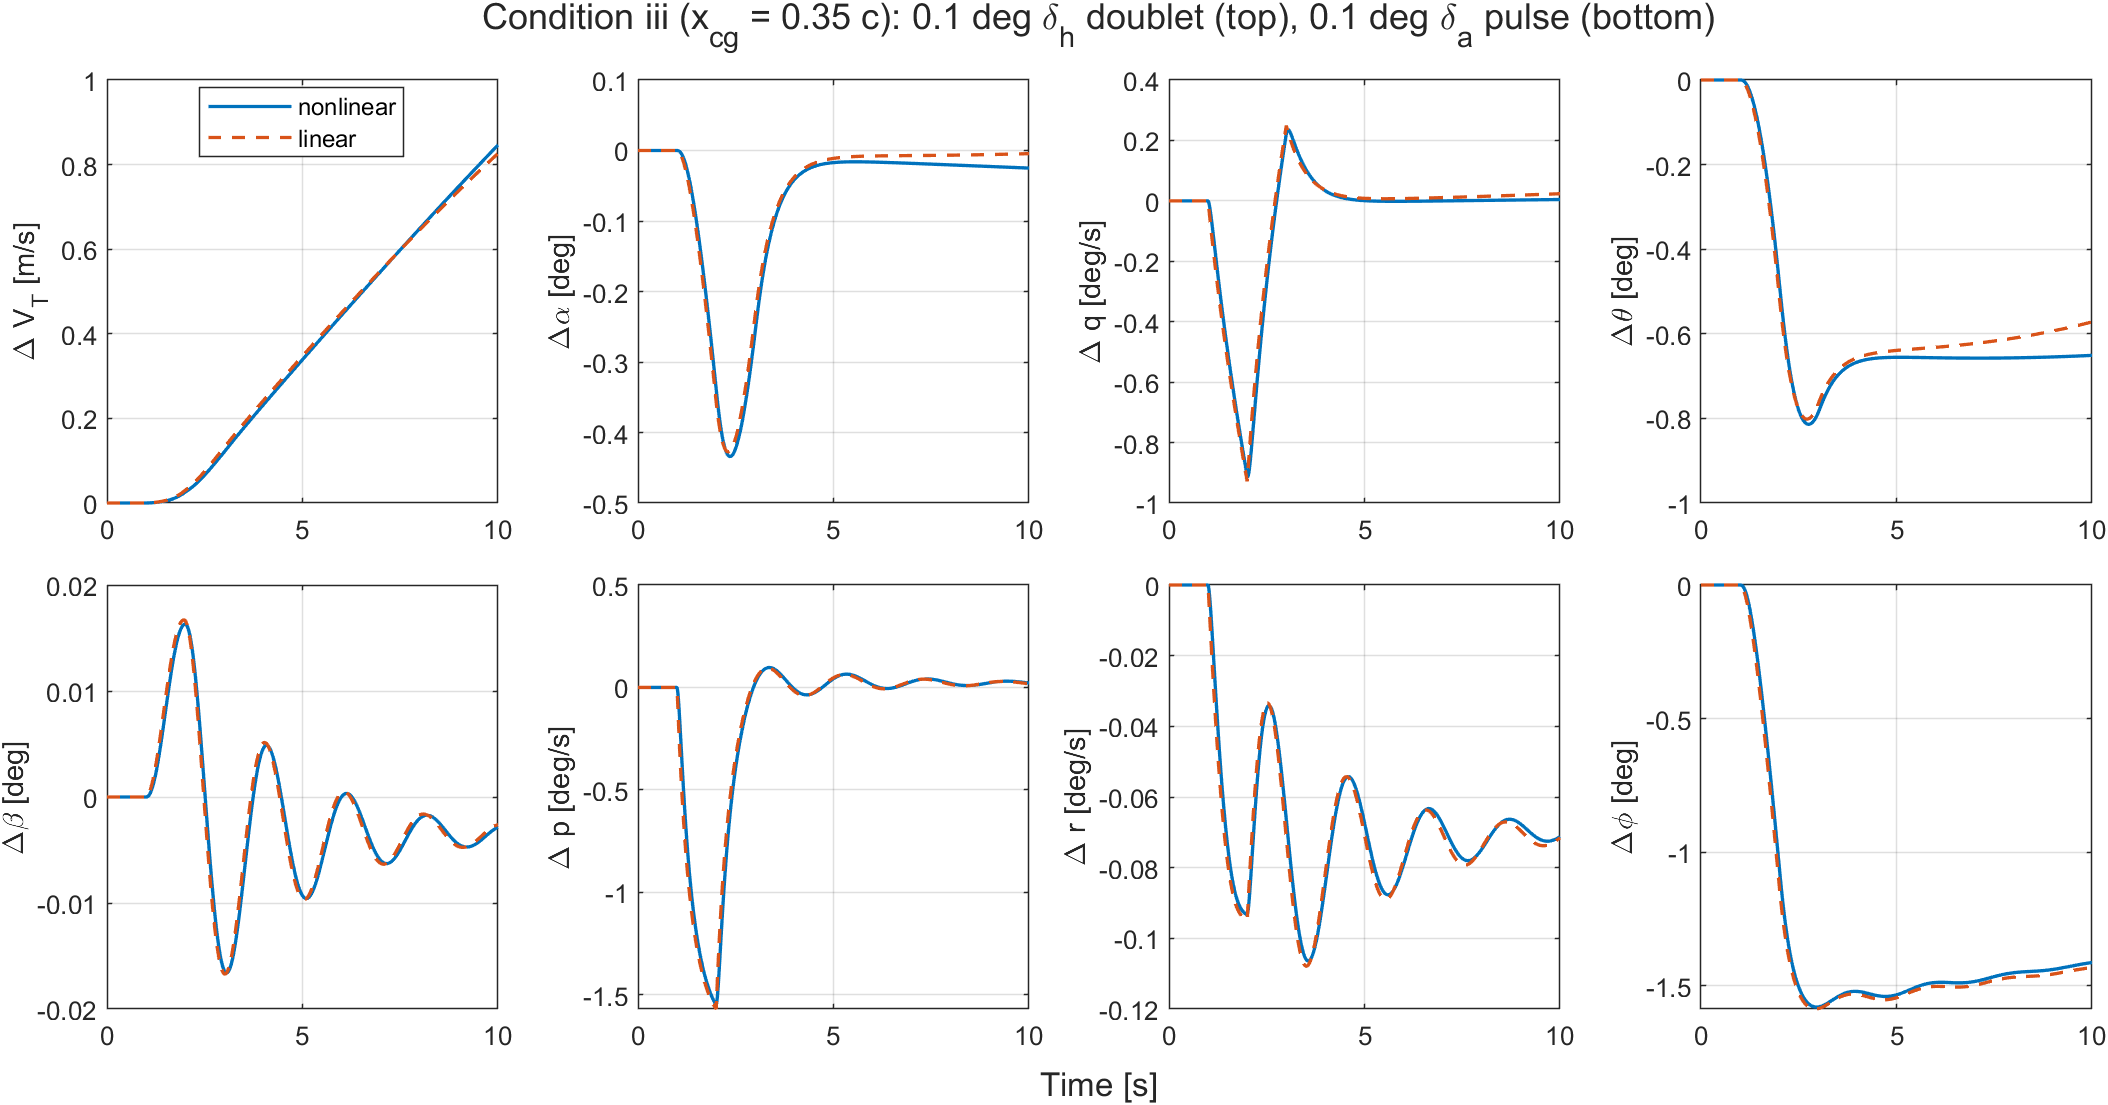
\includegraphics[width=0.95\textwidth]{figures/HW2_LinVsNonlin_iii.png}
\caption{Linear (dashed, scheduled LEF) and nonlinear (solid) responses in condition iii: $0.1^\circ$ stabilator doublet (top) and $0.1^\circ$ aileron pulse (bottom).}
\label{fig:linnl}
\end{figure}

\emph{Corrections to Homework 2.} After the Homework 2 feedback:
\begin{enumerate}
\item the load factor of case 5 is now $1/\cos\mu$ (Lecture 4); before, the body-axis normal acceleration was used, which gave $1/\cos\mu=4.058$. The new trim has $\phi=75.74^\circ$ instead of $75.95^\circ$ (Table~\ref{tab:trim});
\item the linearization lets $\delta_{lef}$ follow its schedule (it was held at the trim value); \texttt{A\_Body}, \texttt{B\_Body}, \texttt{A\_Wind} and \texttt{B\_Wind} were recomputed;
\item the comparison of the three linear models now explains each change (above);
\item the code was simplified: the trim, linearization and simulation are short functions, and the extra checks of Homework 2 were removed;
\item two conventions of the Homework 2 solution manual were adopted: the mass $m=9295.4$~kg (before, $W/g_0=9298.64$~kg) and the step of $10^{-3}$ of Lecture~5 (before, $10^{-4}$ scaled by $V_T$).
\end{enumerate}
With these, the results agree with the solution manual. Every trim quantity is equal to the manual's or differs by one or two units in its last digit (case 5: $\alpha=0.17666$ vs.\ $0.17667$~rad, $\delta_T=81.129$ vs.\ $81.131$\,\%), and $\mu=59.922^\circ$ and $75.522^\circ$ in cases 4 and 5 are the same. Most entries of the linear models agree to the last printed digit; the only differences, of order $10^{-4}$, are in the derivatives with respect to $\beta$ (e.g., $a_{15}=0.0482$ vs.\ $0.0488$ at condition i). The aerodynamic tables have a kink at $\beta=0$, so the central difference averages the two slopes and depends slightly on the small numerical $\beta$ left at trim.
All results were also recomputed with the revised model of Sec.~II.C, whose $g$ is 0.1\,\% smaller at 10\,000~ft; this changes the trim angles by at most $0.01^\circ$. \texttt{run\_MT.m} repeats the trim and linearization at conditions i, ii and iii and reproduces the matrices of \texttt{HW2\_Group2.mat} exactly.

\section{Trimmed-Flight Simulation}

\subsection{Method}
The nonlinear model is started from each trim point: the rigid-body states from the trim solution, the actuator states at the trim deflections, the engine power at the steady-state level of the trim throttle, and the LEF filter at steady state. The stabilator, aileron, rudder and throttle commands are held at their trim values, and $\delta_{lef}$ follows the schedule. The model is integrated with its variable-step solver (maximum step 0.01~s) and the results are resampled at 0.01~s for \texttt{Sim\_i}, \texttt{Sim\_ii} and \texttt{Sim\_iii}. Conditions i and iii run for 60~s; condition ii runs until the heading has changed by $360^\circ$.

\subsection{Results}
Figures~\ref{fig:sim_i}--\ref{fig:sim_iii} show the time histories, and Table~\ref{tab:sim} lists the largest deviations from trim. The control inputs stay at their trim values throughout.

\begin{table}[hbt!]
\caption{\label{tab:sim} Largest deviations from trim during the simulations (angles in deg, rates in deg/s)}
\centering
\begin{tabular}{ccccccccc}
\toprule
Condition & Duration [s] & $|\Delta V_T|$ [m/s] & $|\Delta\alpha|$ & $|\Delta\beta|$ & $|\Delta\phi|$ & $|\Delta\theta|$ & $|\Delta q|$ & $|\Delta h|$ [m] \\
\midrule
\tabinput{tables/sim.tex}
\bottomrule
\end{tabular}
\end{table}

\emph{Condition i.} The trim holds: in 60~s the speed changes by less than $4\times10^{-4}$~m/s, the attitude by about $10^{-4}$~deg and the altitude by 1~cm. The small residual motion shows the modes of Sec.~VI. $V_T$, $\theta$ and $h$ oscillate slowly with a half period of about 45~s, which is the phugoid (period 88~s). The roll and yaw rates show a decaying oscillation in the first 10~s with a period of about 1.8~s, which is the Dutch roll (1.84~s). The bank angle drifts monotonically on the time scale of the stable spiral mode ($\tau=89$~s). The motion is excited by the trim residuals and the solver start-up; all modes are stable, so it stays bounded.

\emph{Condition ii.} One full turn takes 73.05~s, against $2\pi/\dot\psi_1=73.04$~s from the trim solution. The ground track (Fig.~\ref{fig:track}) is a closed circle of radius 2289~m, compared with $V_T^2/(g\tan\phi)=2285$~m, and the altitude changes by 9~cm. The pitch attitude and yaw rate oscillate with a period of about 50~s, close to the 57~s period of the coupled phugoid--spiral mode of the full model (Sec.~VI); the Dutch-roll transient again decays within 10~s.

\emph{Condition iii.} The deviations grow monotonically instead of oscillating: the pitch angle changes by $5.1\times10^{-4}$, $1.7\times10^{-3}$ and $3.9\times10^{-3}$~deg at 20, 40 and 60~s, while the aircraft slowly pitches down, accelerates and descends. The growth rate between 40 and 60~s is about 0.04~s$^{-1}$. This agrees with the unstable phugoid of the linear model with the scheduled LEF (Sec.~VI), $\lambda=0.034\pm0.083j$~s$^{-1}$ with $t_2=20.5$~s; its 76~s period is longer than the run, so the motion looks monotonic. The remaining difference in growth rate comes from the altitude and engine states, which the 8-state model omits. The fixed-LEF root $+0.787$~s$^{-1}$ would amplify a disturbance by a factor of $e^{47}$ in 60~s; it does not appear because the flap schedule is active in the simulation. The trim of condition iii is therefore an unstable equilibrium; the deviations remain small only because the initial disturbance is of the order of the trim residuals.

\begin{figure}[hbt!]
\centering
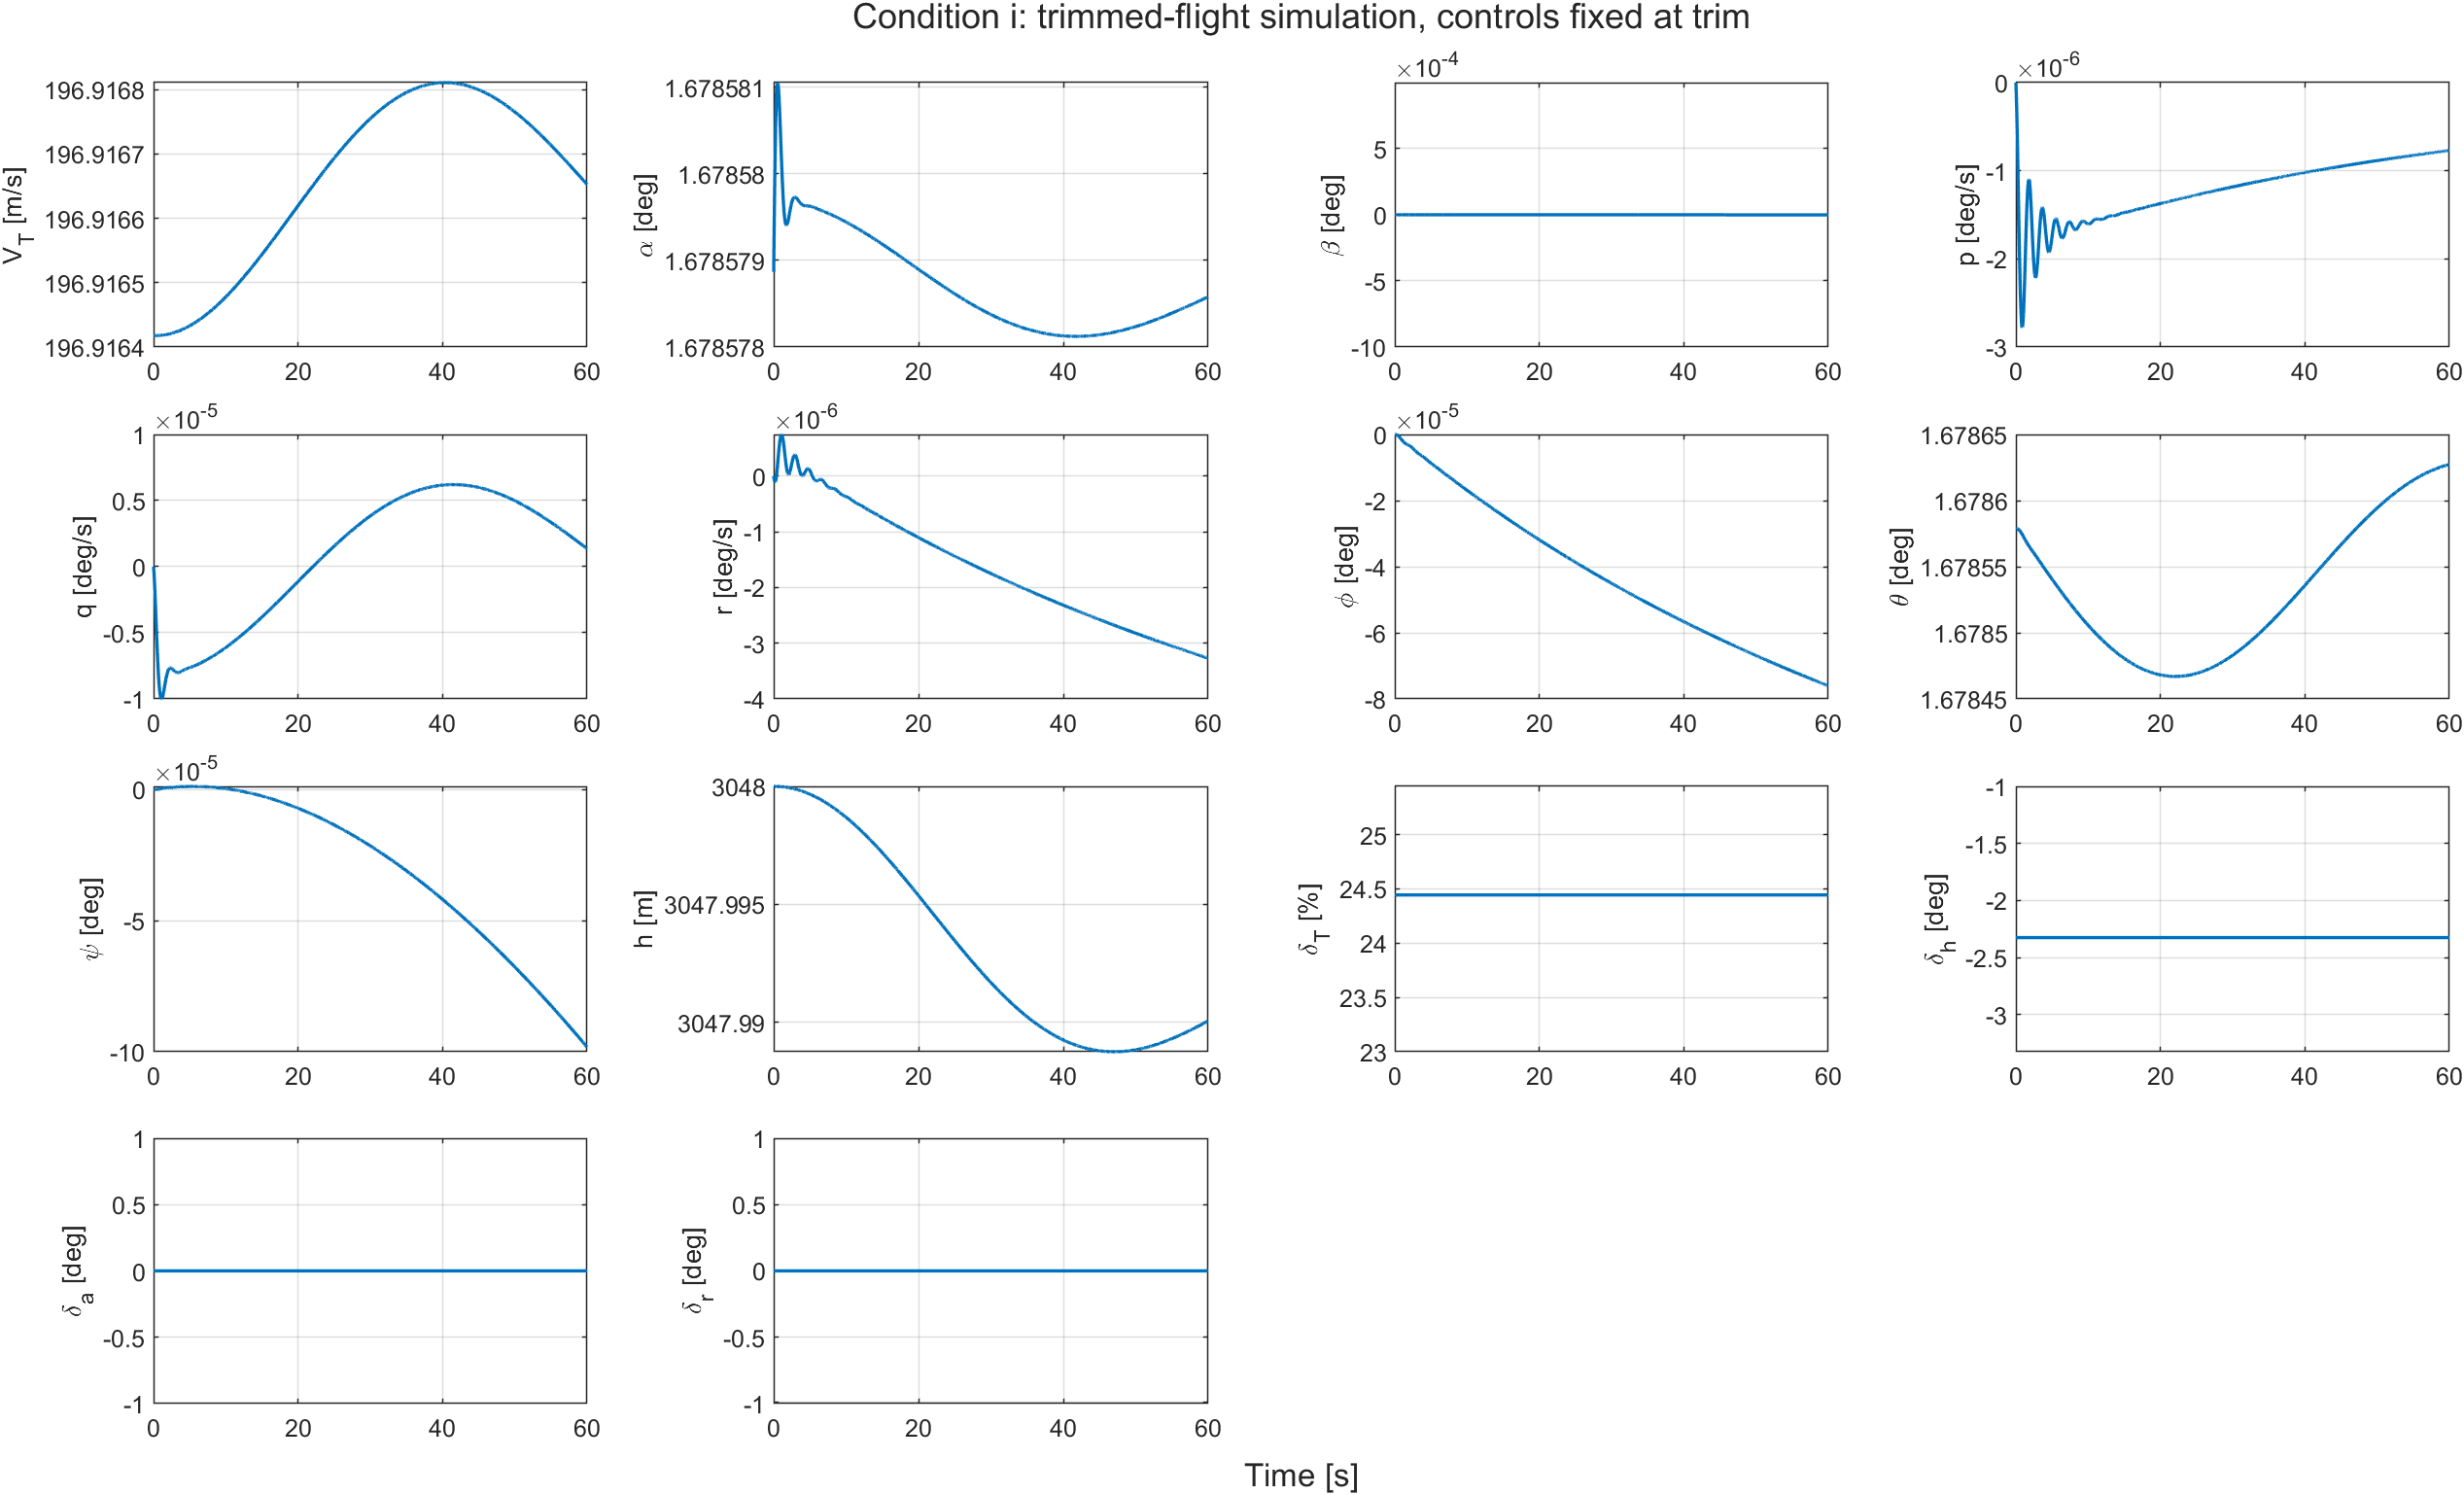
\includegraphics[width=\textwidth]{figures/MT_Sim_i.png}
\caption{Trimmed-flight simulation, condition i (controls fixed at trim).}
\label{fig:sim_i}
\end{figure}

\begin{figure}[hbt!]
\centering
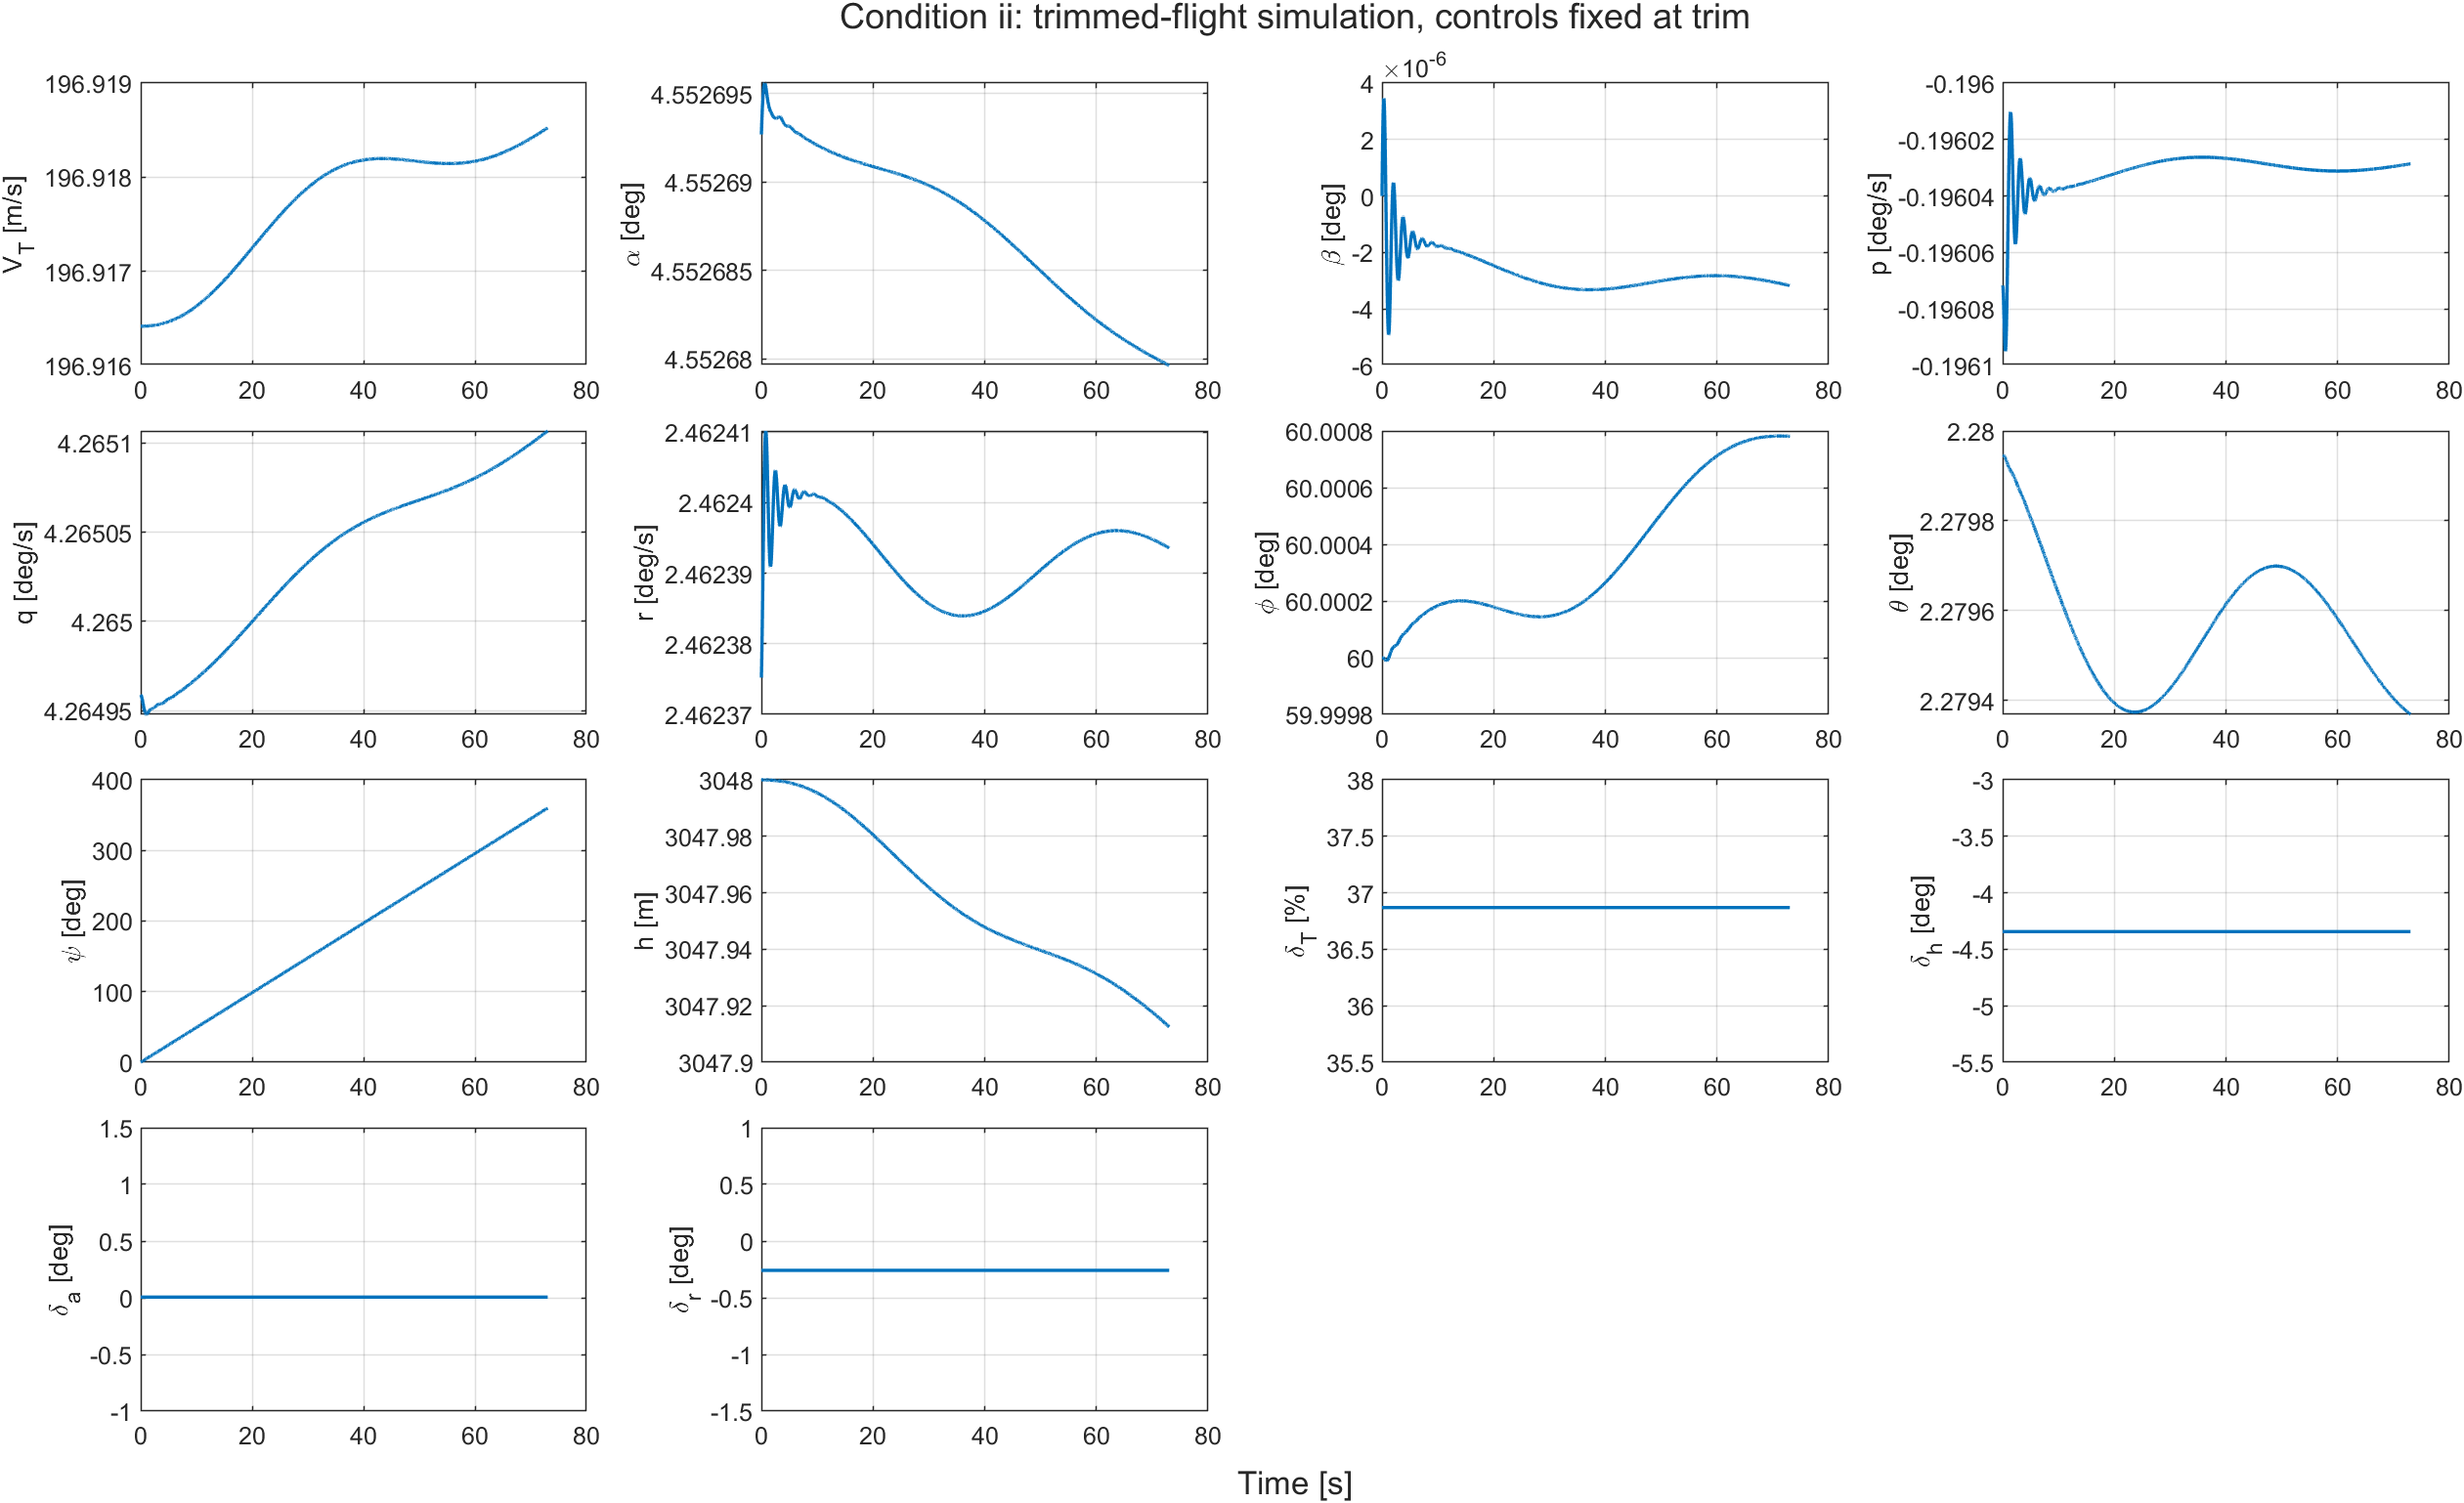
\includegraphics[width=\textwidth]{figures/MT_Sim_ii.png}
\caption{Trimmed-flight simulation, condition ii (one complete turn).}
\label{fig:sim_ii}
\end{figure}

\begin{figure}[hbt!]
\centering
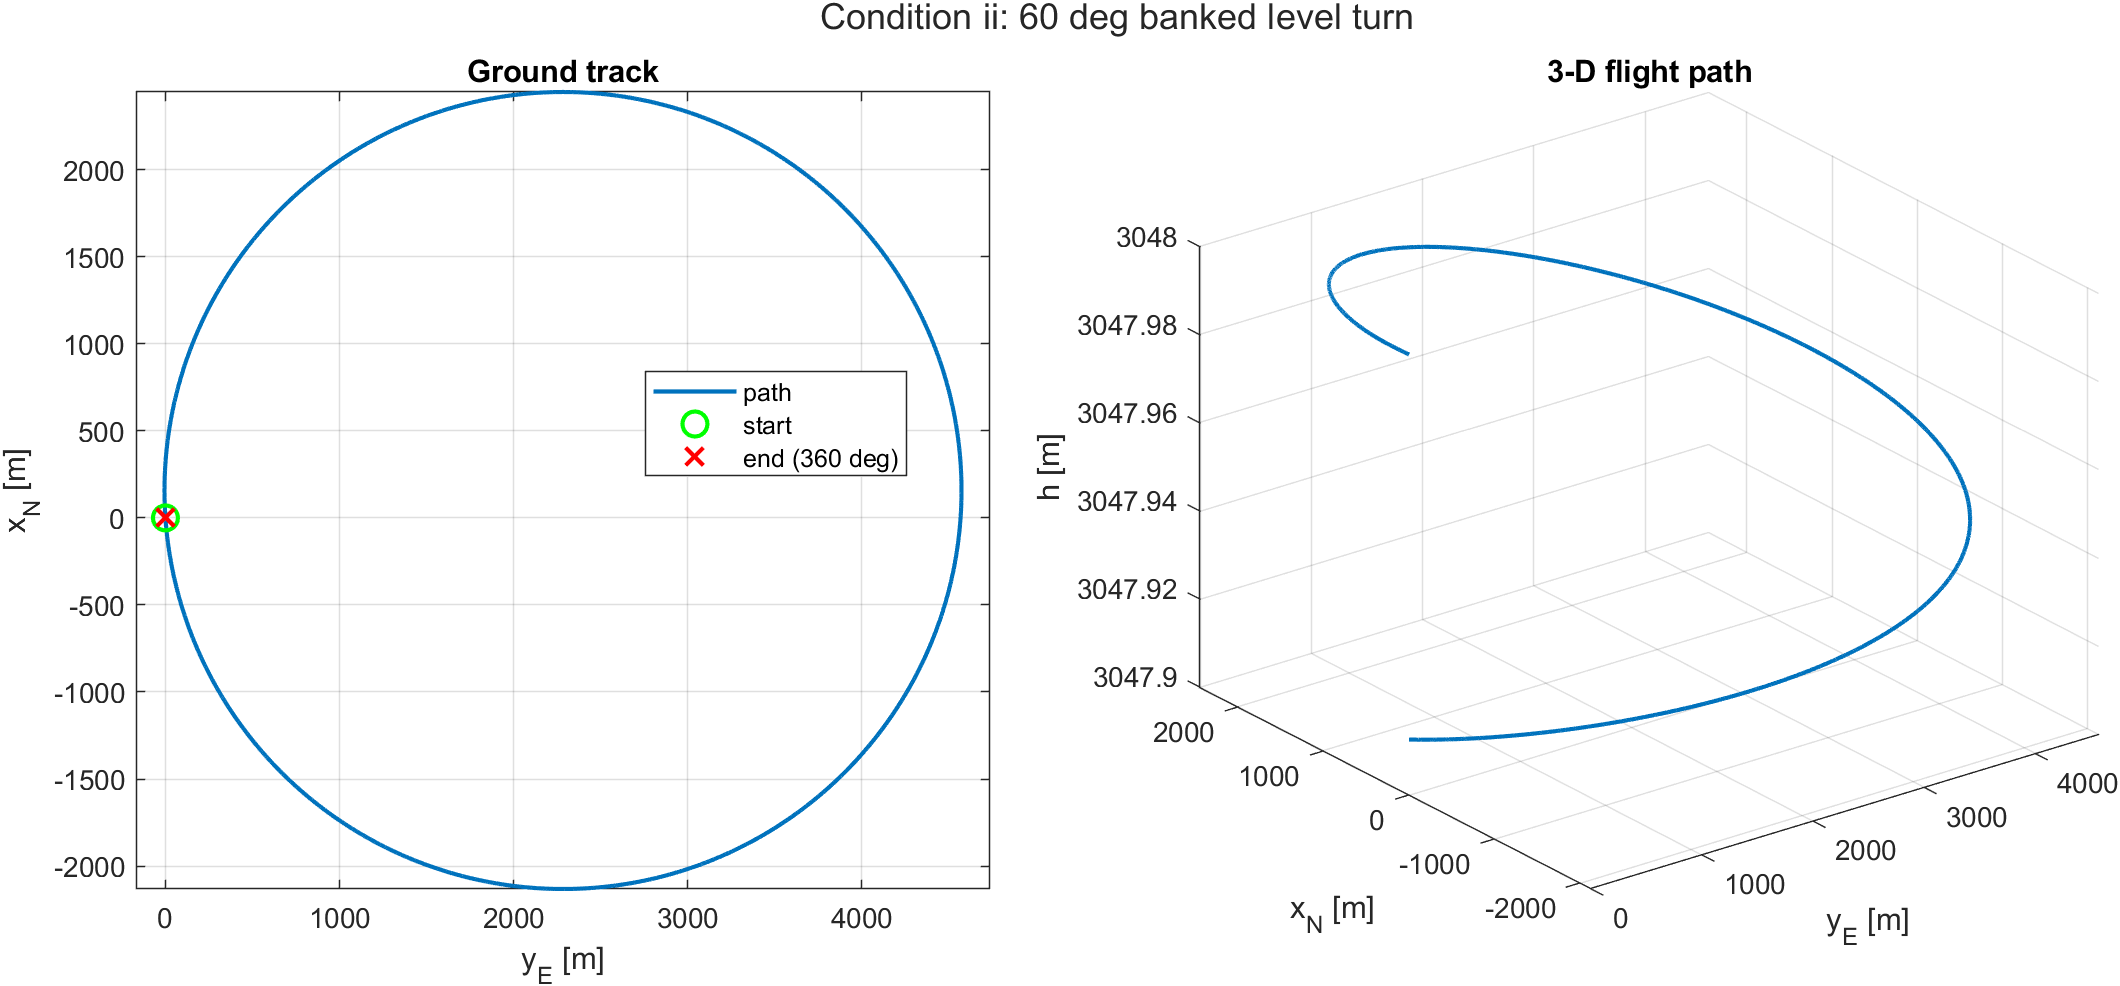
\includegraphics[width=0.85\textwidth]{figures/MT_Track_ii.png}
\caption{Ground track and three-dimensional flight path, condition ii (altitude axis magnified).}
\label{fig:track}
\end{figure}

\begin{figure}[hbt!]
\centering
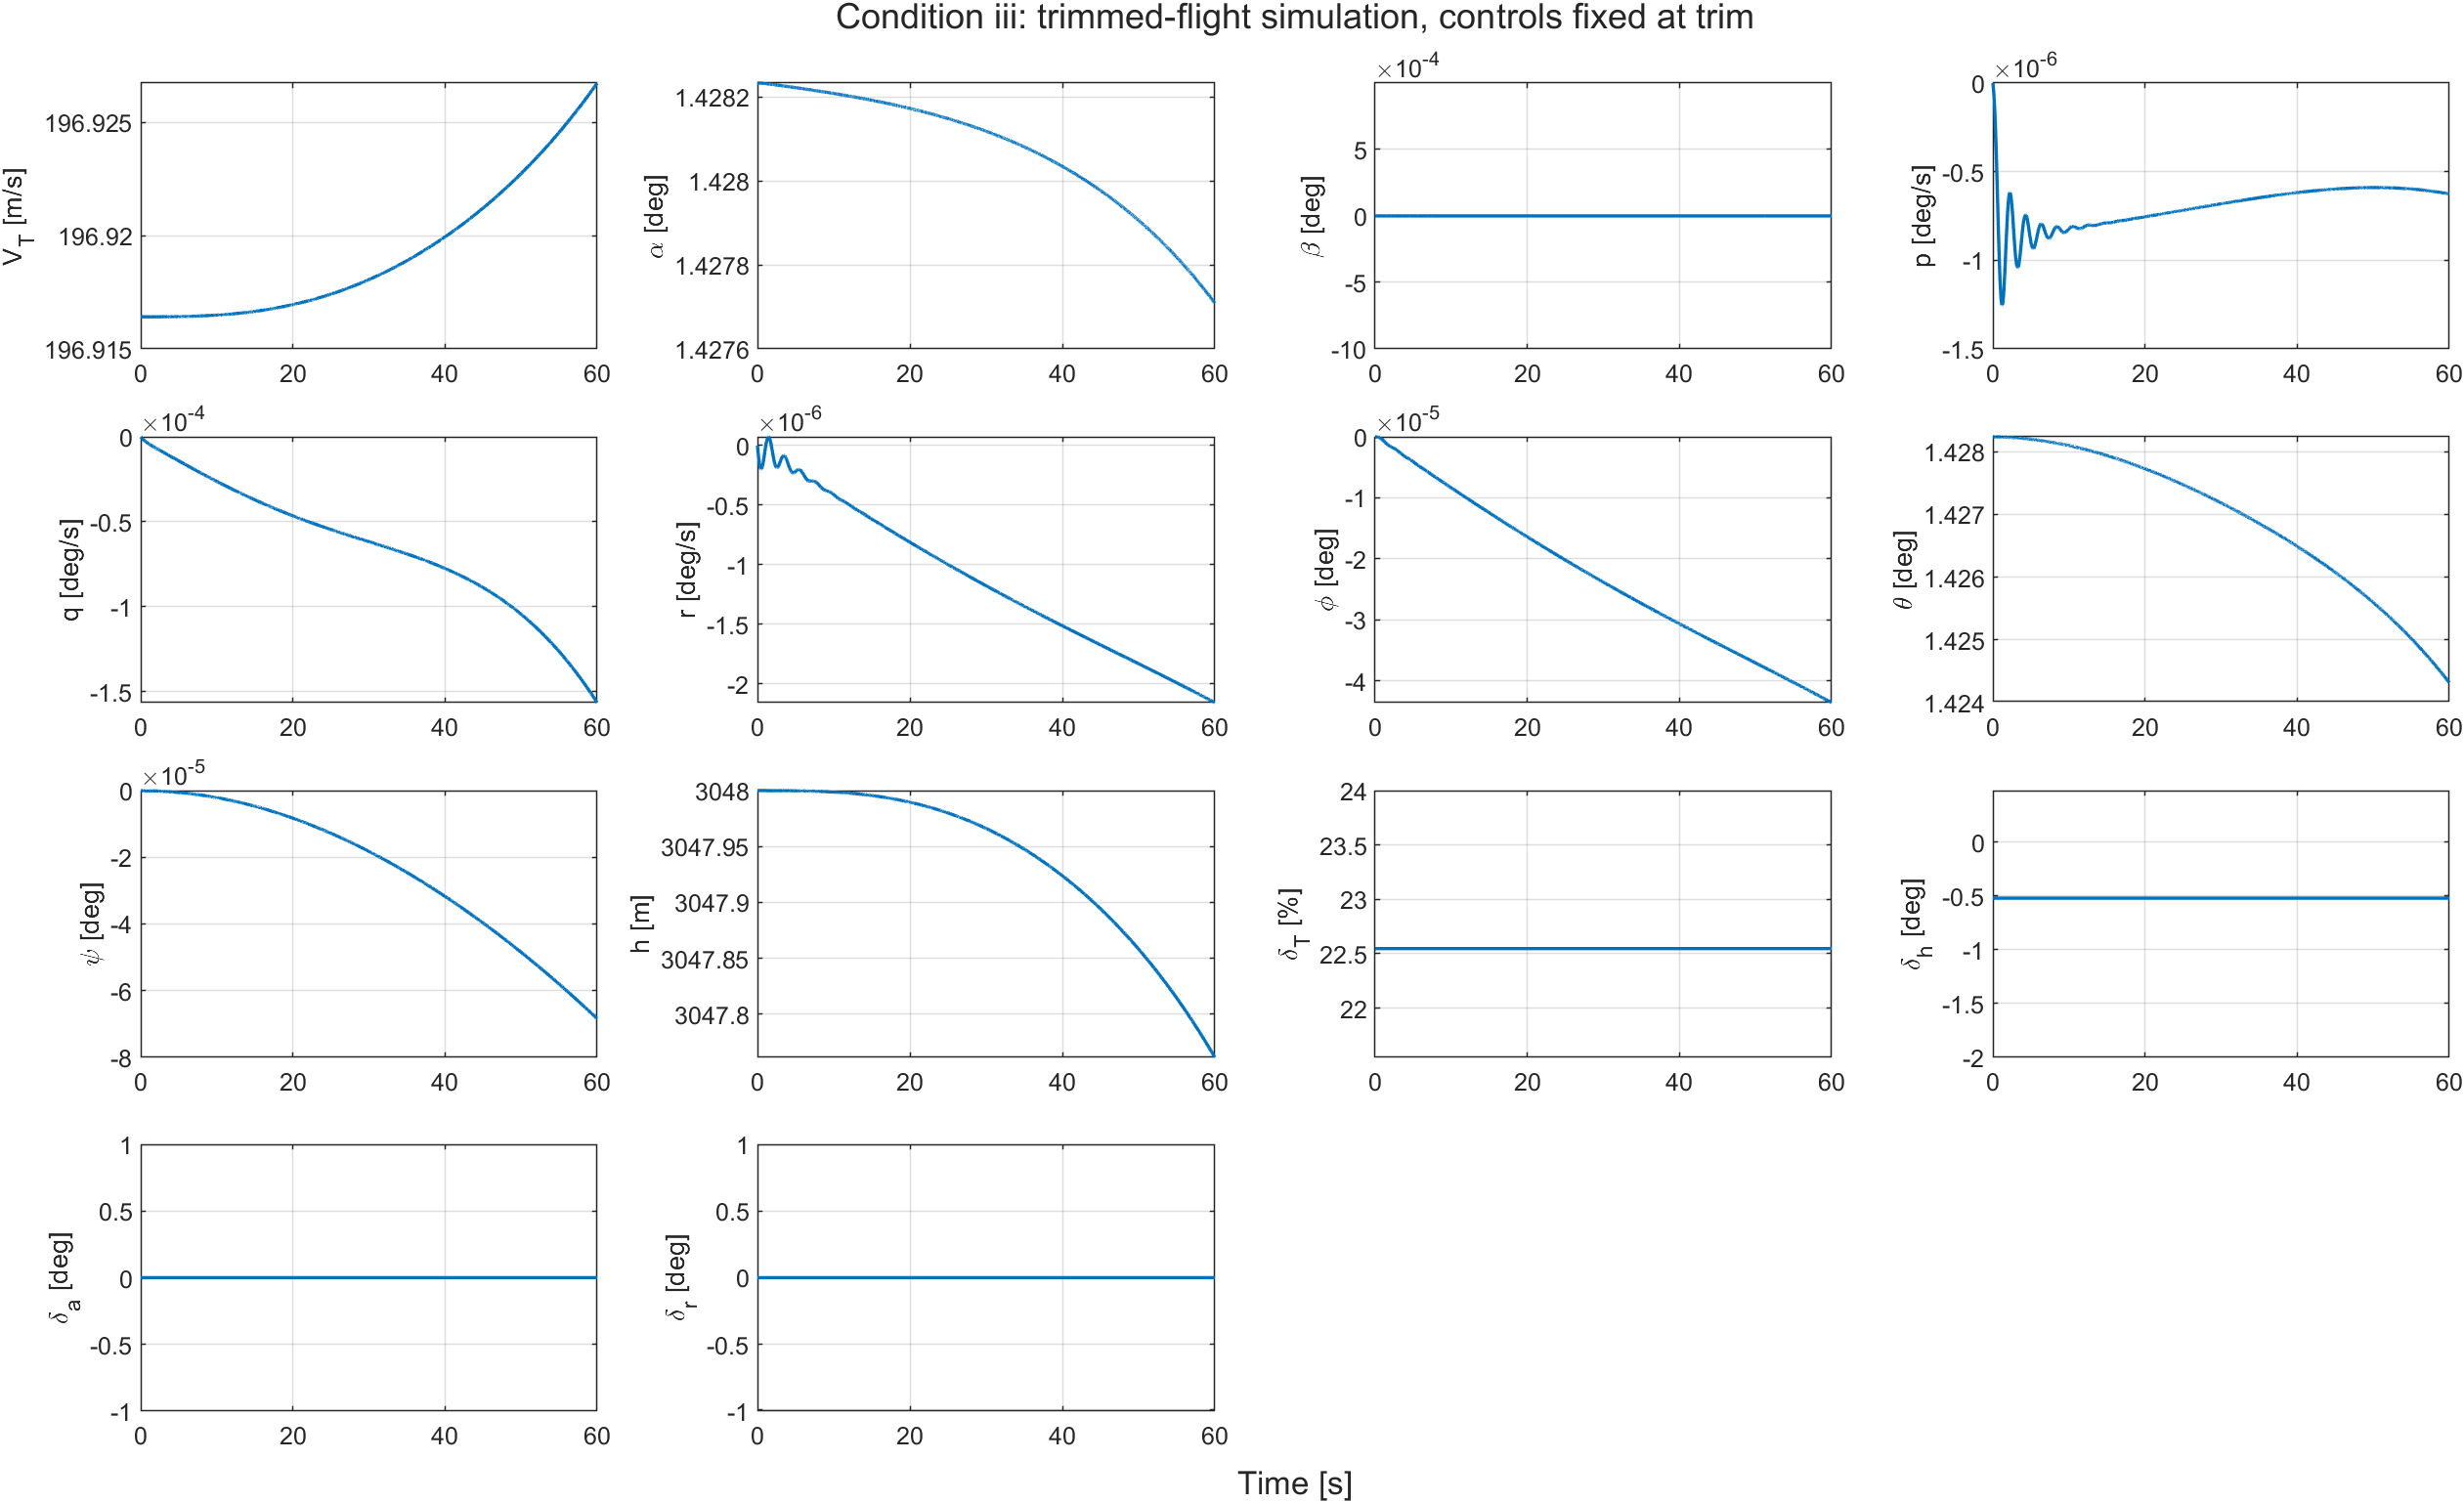
\includegraphics[width=\textwidth]{figures/MT_Sim_iii.png}
\caption{Trimmed-flight simulation, condition iii (controls fixed at trim).}
\label{fig:sim_iii}
\end{figure}

\section{Stability Parameters}

\subsection{Relations}
As specified for Problem 2, this section uses the wind-axis matrix with $\delta_{lef}$ held at its trim value, so that $A$ contains the derivatives of the airframe alone; with the schedule, $a_{32}$ would also contain the flap moment $\partial C_m/\partial\delta_{lef}\cdot\partial\delta_{lef}/\partial\alpha$ (Sec.~III.B). The longitudinal state variable model of Lecture 6~\cite{lec6} (pp.~24--25), with $\Delta V_T$ in place of $\Delta u$ and $U_1=V_T$ at trim, gives
\begin{equation}
a_{11}=X_u+X_{T_u},\quad
a_{31}=(M_u+M_{T_u})-\frac{M_{\dot\alpha}Z_u}{Z_{\dot\alpha}-U_1},\quad
a_{32}=(M_\alpha+M_{T_\alpha})-\frac{M_{\dot\alpha}Z_\alpha}{Z_{\dot\alpha}-U_1},\quad
a_{33}=M_q-\frac{M_{\dot\alpha}(Z_q+U_1)}{Z_{\dot\alpha}-U_1}.
\end{equation}
In the lateral-directional model (pp.~100--101) the roll and yaw rows contain the inertia coupling,
\begin{equation}
a_{6k}=\frac{L_k+(I_{xz}/I_{xx})N_k}{1-I_{xz}^2/(I_{xx}I_{zz})},\qquad
a_{7k}=\frac{N_k+(I_{xz}/I_{zz})L_k}{1-I_{xz}^2/(I_{xx}I_{zz})},\qquad k=\beta,p,r,
\end{equation}
which is inverted as
\begin{equation}
L_k=a_{6k}-\frac{I_{xz}}{I_{xx}}\,a_{7k},\qquad N_k=a_{7k}-\frac{I_{xz}}{I_{zz}}\,a_{6k}.
\label{eq:invert}
\end{equation}
Since $p$ and $r$ are body-axis rates, the body-axis inertias of Sec.~II are used, and the derivatives are body-axis derivatives. The nondimensional derivatives follow from the definitions of Lecture 5~\cite{lec5} (pp.~116 and 123):
\begin{gather}
X_u=-\frac{\bar q_1S}{mU_1}(C_{D_u}+2C_{D_1}),\quad
M_u=\frac{\bar q_1S\bar c}{I_{yy}U_1}(C_{m_u}+2C_{m_1}),\quad
M_\alpha=\frac{\bar q_1S\bar c}{I_{yy}}C_{m_\alpha},\quad
M_q=\frac{\bar q_1S\bar c^2}{2I_{yy}U_1}C_{m_q},\\
L_\beta=\frac{\bar q_1Sb}{I_{xx}}C_{l_\beta},\quad
N_\beta=\frac{\bar q_1Sb}{I_{zz}}C_{n_\beta},\quad
L_{p,r}=\frac{\bar q_1Sb^2}{2I_{xx}U_1}C_{l_{p,r}},\quad
N_{p,r}=\frac{\bar q_1Sb^2}{2I_{zz}U_1}C_{n_{p,r}}.
\end{gather}
At all three conditions $U_1=196.92$~m/s and $\bar q_1=17\,564$~Pa.

\emph{Thrust.} The thrust acts along the body $x$ axis, so its contribution to $\dot V_T$ is $T\cos\alpha\cos\beta/m$ and
\begin{equation}
X_{T_u}=\frac{\cos\alpha_1\cos\beta_1}{m}\frac{\partial T}{\partial V_T}\bigg|_{\delta_T,h}.
\end{equation}
The derivative is computed by running the Propulsion block of the plant model alone, at the trim throttle and altitude and with the engine at steady state, at $M=0.6\pm0.001$. Then $X_u=a_{11}-X_{T_u}$.

\emph{Trim coefficients.} From the $\dot V_T$ equation at trim, $C_{D_1}=(T_1\cos\alpha_1\cos\beta_1-mg\sin\gamma_1)/(\bar q_1S)$, and $C_{L_1}=(mg\cos\gamma_1/\cos\phi_1-T_1\sin\alpha_1)/(\bar q_1S)$. In straight flight the aerodynamic pitching moment is zero at trim, $C_{m_1}=0$. In the turn it balances the inertial and gyroscopic moments, $C_{m_1}=[\boldsymbol\omega_1\times(\mathbf I\boldsymbol\omega_1+\mathbf h_E)]_y/(\bar q_1S\bar c)=1.0\times10^{-5}$, which is negligible and is taken as zero. Table~\ref{tab:p2trim} lists these quantities, Table~\ref{tab:aelem} the elements of $A$ that were used, and Tables~\ref{tab:params} and~\ref{tab:derivs} the results.

\begin{table}[hbt!]
\caption{\label{tab:p2trim} Trim quantities used for the derivatives}
\centering
\begin{tabular}{ccccc}
\toprule
Condition & $T_1$ [N] & $\partial T/\partial V_T$ [N\,s/m] & $C_{L_1}$ & $C_{D_1}$ \\
\midrule
\tabinput{tables/p2trim.tex}
\bottomrule
\end{tabular}
\end{table}

\begin{table}[hbt!]
\caption{\label{tab:aelem} Elements of the wind-axis matrix $A$ used in Problem 2 ($\delta_{lef}$ fixed)}
\centering
\begin{tabular}{llccc}
\toprule
Element & Unit & i & ii & iii \\
\midrule
\tabinput{tables/aelem.tex}
\bottomrule
\end{tabular}
\end{table}

\begin{table}[hbt!]
\caption{\label{tab:params} Stability parameters (\texttt{StabParams})}
\centering
\begin{tabular}{llccc}
\toprule
Parameter & Unit & i & ii & iii \\
\midrule
\tabinput{tables/params.tex}
\bottomrule
\end{tabular}
\end{table}

\begin{table}[hbt!]
\caption{\label{tab:derivs} Nondimensional stability derivatives (\texttt{StabDerivs}, rad$^{-1}$) and normal signs~\cite{lec5}}
\centering
\begin{tabular}{lcccc}
\toprule
Derivative & i & ii & iii & Normal sign \\
\midrule
\tabinput{tables/derivs.tex}
\bottomrule
\end{tabular}
\end{table}

\subsection{Terms that are zero in the model}
\begin{itemize}
\item $Z_{\dot\alpha}=M_{\dot\alpha}=0$: the TP-1538 data contain no $\dot\alpha$ derivatives, so the correction terms in $a_{31}$, $a_{32}$ and $a_{33}$ vanish and $a_{32}=M_\alpha+M_{T_\alpha}$, $a_{33}=M_q$.
\item $M_{T_u}=M_{T_\alpha}=0$ and $N_{T_\beta}=0$: the thrust acts along the body $x$ axis through the center of gravity and does not depend on $\alpha$ or $\beta$; the engine model has no inlet momentum terms.
\item $C_{D_u}$ and $C_{m_u}$ vanish in straight flight (i and iii, of order $10^{-9}$, i.e., numerical zero): the aerodynamic tables do not depend on Mach number, so a speed change at constant $\alpha$ only scales the forces and moments with $\bar q$, which the $2C_{D_1}$ and $2C_{m_1}$ terms already contain. For the same reason $C_{m_1}=0$ in straight flight, where the aerodynamic moment alone is balanced.
\item $X_{T_u}$ is not zero: at this condition the thrust decreases slightly with Mach number ($\partial T/\partial V_T\approx-35$~N\,s/m), so the engine adds about 23\,\% to the speed damping in condition i.
\end{itemize}
Conversely, the lecture model assumes $C_{D_q}\approx0$ (zero $X_q$), but the F-16 data contain rate terms in the axial force, and the element $a_{13}=\partial\dot V_T/\partial q=-0.138$~m/s per rad/s is not zero.

\subsection{Signs and static stability}
All derivatives have their normal signs in conditions i and ii, and the derivatives with an undefined normal sign ($C_{D_u}$, $C_{m_u}$, $C_{n_p}$) are small. In condition iii, $C_{m_\alpha}=+0.156$~rad$^{-1}$ has the wrong sign. The aircraft is therefore
\begin{itemize}
\item statically stable in pitch, roll and yaw at conditions i and ii ($C_{m_\alpha}<0$, $C_{l_\beta}<0$, $C_{n_\beta}>0$);
\item statically unstable in pitch at condition iii, but stable in roll and yaw.
\end{itemize}
The difference between i and iii is the moment transfer of Sec.~II, $C_m\leftarrow C_m+C_Z(0.35-x_{cg})$, which vanishes at $x_{cg}=0.35$. It shifts $C_{m_\alpha}$ by $0.10\,C_{Z_\alpha}=-0.386$~rad$^{-1}$, so $C_{Z_\alpha}\approx-3.86$~rad$^{-1}$, and places the neutral point at about $0.35-0.156/3.86\approx0.31\bar c$, consistent with the static margin of $-4\,\%\,\bar c$ found in Homework 1. The same term adds $0.10\,C_{Z_q}$ to $C_{m_q}$, which explains the larger pitch damping at the forward center of gravity ($-8.22$ against $-5.23$). The shorter vertical-tail moment arm at $0.35\bar c$ reduces $C_{n_\beta}$ from 0.219 to 0.181.

\subsection{Condition ii}
The relations of Lecture 5 are derived for steady straight flight with $p_1=q_1=r_1=\phi_1=0$ (pp.~13 and 16). In the turn the values differ for three reasons.

\emph{Aerodynamic state.} The trim angle of attack is $4.55^\circ$ instead of $1.68^\circ$ and $\delta_{lef}=5.45^\circ$ instead of $1.49^\circ$, so the tables are read at a different point. The dihedral effect grows with $\alpha$ ($C_{l_\beta}$ from $-0.102$ to $-0.134$), and so does $C_{l_r}$, which scales with the lift.

\emph{Inertial terms.} With $\boldsymbol\omega_1\neq0$, the inertial term $\boldsymbol\omega\times\mathbf I\boldsymbol\omega$ of Eq.~(\ref{eq:eom}) and the engine moment $\mathbf M_T$, together $\boldsymbol\omega\times(\mathbf I\boldsymbol\omega+\mathbf h_E)$, have a nonzero Jacobian with respect to $p$, $q$ and $r$, which appears in the rate columns of $A$ together with the aerodynamic damping. Equation~(\ref{eq:invert}) removes the $I_{xz}$ coupling but not these terms. The largest is $\partial[\boldsymbol\omega\times\mathbf I\boldsymbol\omega]_z/\partial p=(I_{yy}-I_{xx})q_1=4.67\times10^{3}$~N\,m\,s, which changes the sign of $C_{n_p}$. Adding the Jacobian back to $\mathbf I A$ gives the aerodynamic part alone (Table~\ref{tab:turnaero}); \texttt{StabDerivs} contains the values obtained from $A$ as specified.

\emph{Rate terms at trim.} A speed change at constant $q_1$ changes $\hat q_1=q_1\bar c/(2U_1)$, so the rate-damping terms make $C_{m_u}$ and $C_{D_u}$ nonzero: $C_{m_u}=-C_{m_q}\hat q_1=8.37\times6.52\times10^{-4}=0.0055$, as in Table~\ref{tab:derivs}.

\begin{table}[hbt!]
\caption{\label{tab:turnaero} Rate derivatives in condition ii: from $A$ and aerodynamic part only (rad$^{-1}$)}
\centering
\begin{tabular}{lcccc}
\toprule
 & $C_{l_p}$ & $C_{n_p}$ & $C_{l_r}$ & $C_{n_r}$ \\
\midrule
\tabinput{tables/turnaero.tex}
\bottomrule
\end{tabular}
\end{table}

\section{Dynamic Modes}

\subsection{Method}
The eigenvalues of the full wind-axis matrix $A$ with the scheduled LEF (\texttt{A\_Wind} of Sec.~III) and of its blocks $A_{11}$ and $A_{22}$ are computed at each condition. For a complex pair $\lambda=-\zeta\omega_n\pm j\omega_n\sqrt{1-\zeta^2}$, $\omega_n=|\lambda|$, $\zeta=-\operatorname{Re}\lambda/|\lambda|$, the period is $2\pi/|\operatorname{Im}\lambda|$ and $\tau=-1/\operatorname{Re}\lambda$; for a real root $\tau=-1/\lambda$. The times to half and to double amplitude are $t_{1/2}=\tau\ln2$ ($\tau>0$) and $t_2=-\tau\ln2$ ($\tau<0$)~\cite{lec6}. In the full model the modes are identified from the eigenvectors: with $\Delta V_T$ scaled by $1/U_1$, the longitudinal share of an eigenvector is the fraction of its squared norm in the first four states, and the four roots with the largest share are taken as longitudinal. Of the longitudinal roots, the one with the largest magnitude is the short period and the remaining complex pair is the phugoid. Of the lateral-directional roots, the complex pair is the Dutch roll, and the faster and slower real roots are the roll and spiral modes. The decoupled blocks are classified in the same way.

\begin{table}[hbt!]
\caption{\label{tab:modes} Modes of the full $8\times8$ model (\texttt{Modes\_Full}); times in s, $\omega_n$ in rad/s}
\centering
\small
\begin{tabular}{cllcccccc}
\toprule
Cond. & Mode & $\lambda$ [s$^{-1}$] & $\omega_n$ & $\zeta$ & Period & $\tau$ & $t_{1/2}$ & $t_2$ \\
\midrule
\tabinput{tables/modes.tex}
\bottomrule
\multicolumn{9}{l}{\footnotesize $^a$The short period splits into two real roots, $-1.978$ and $-0.0751$~s$^{-1}$; the faster one is entered.}
\end{tabular}
\end{table}

\begin{table}[hbt!]
\caption{\label{tab:modesdec} Modes of the decoupled blocks $A_{11}$ and $A_{22}$ in condition ii (\texttt{Modes\_Dec})}
\centering
\small
\begin{tabular}{llcccccc}
\toprule
Mode & $\lambda$ [s$^{-1}$] & $\omega_n$ & $\zeta$ & Period & $\tau$ & $t_{1/2}$ & $t_2$ \\
\midrule
\tabinput{tables/modesdec.tex}
\bottomrule
\end{tabular}
\end{table}

\begin{figure}[hbt!]
\centering
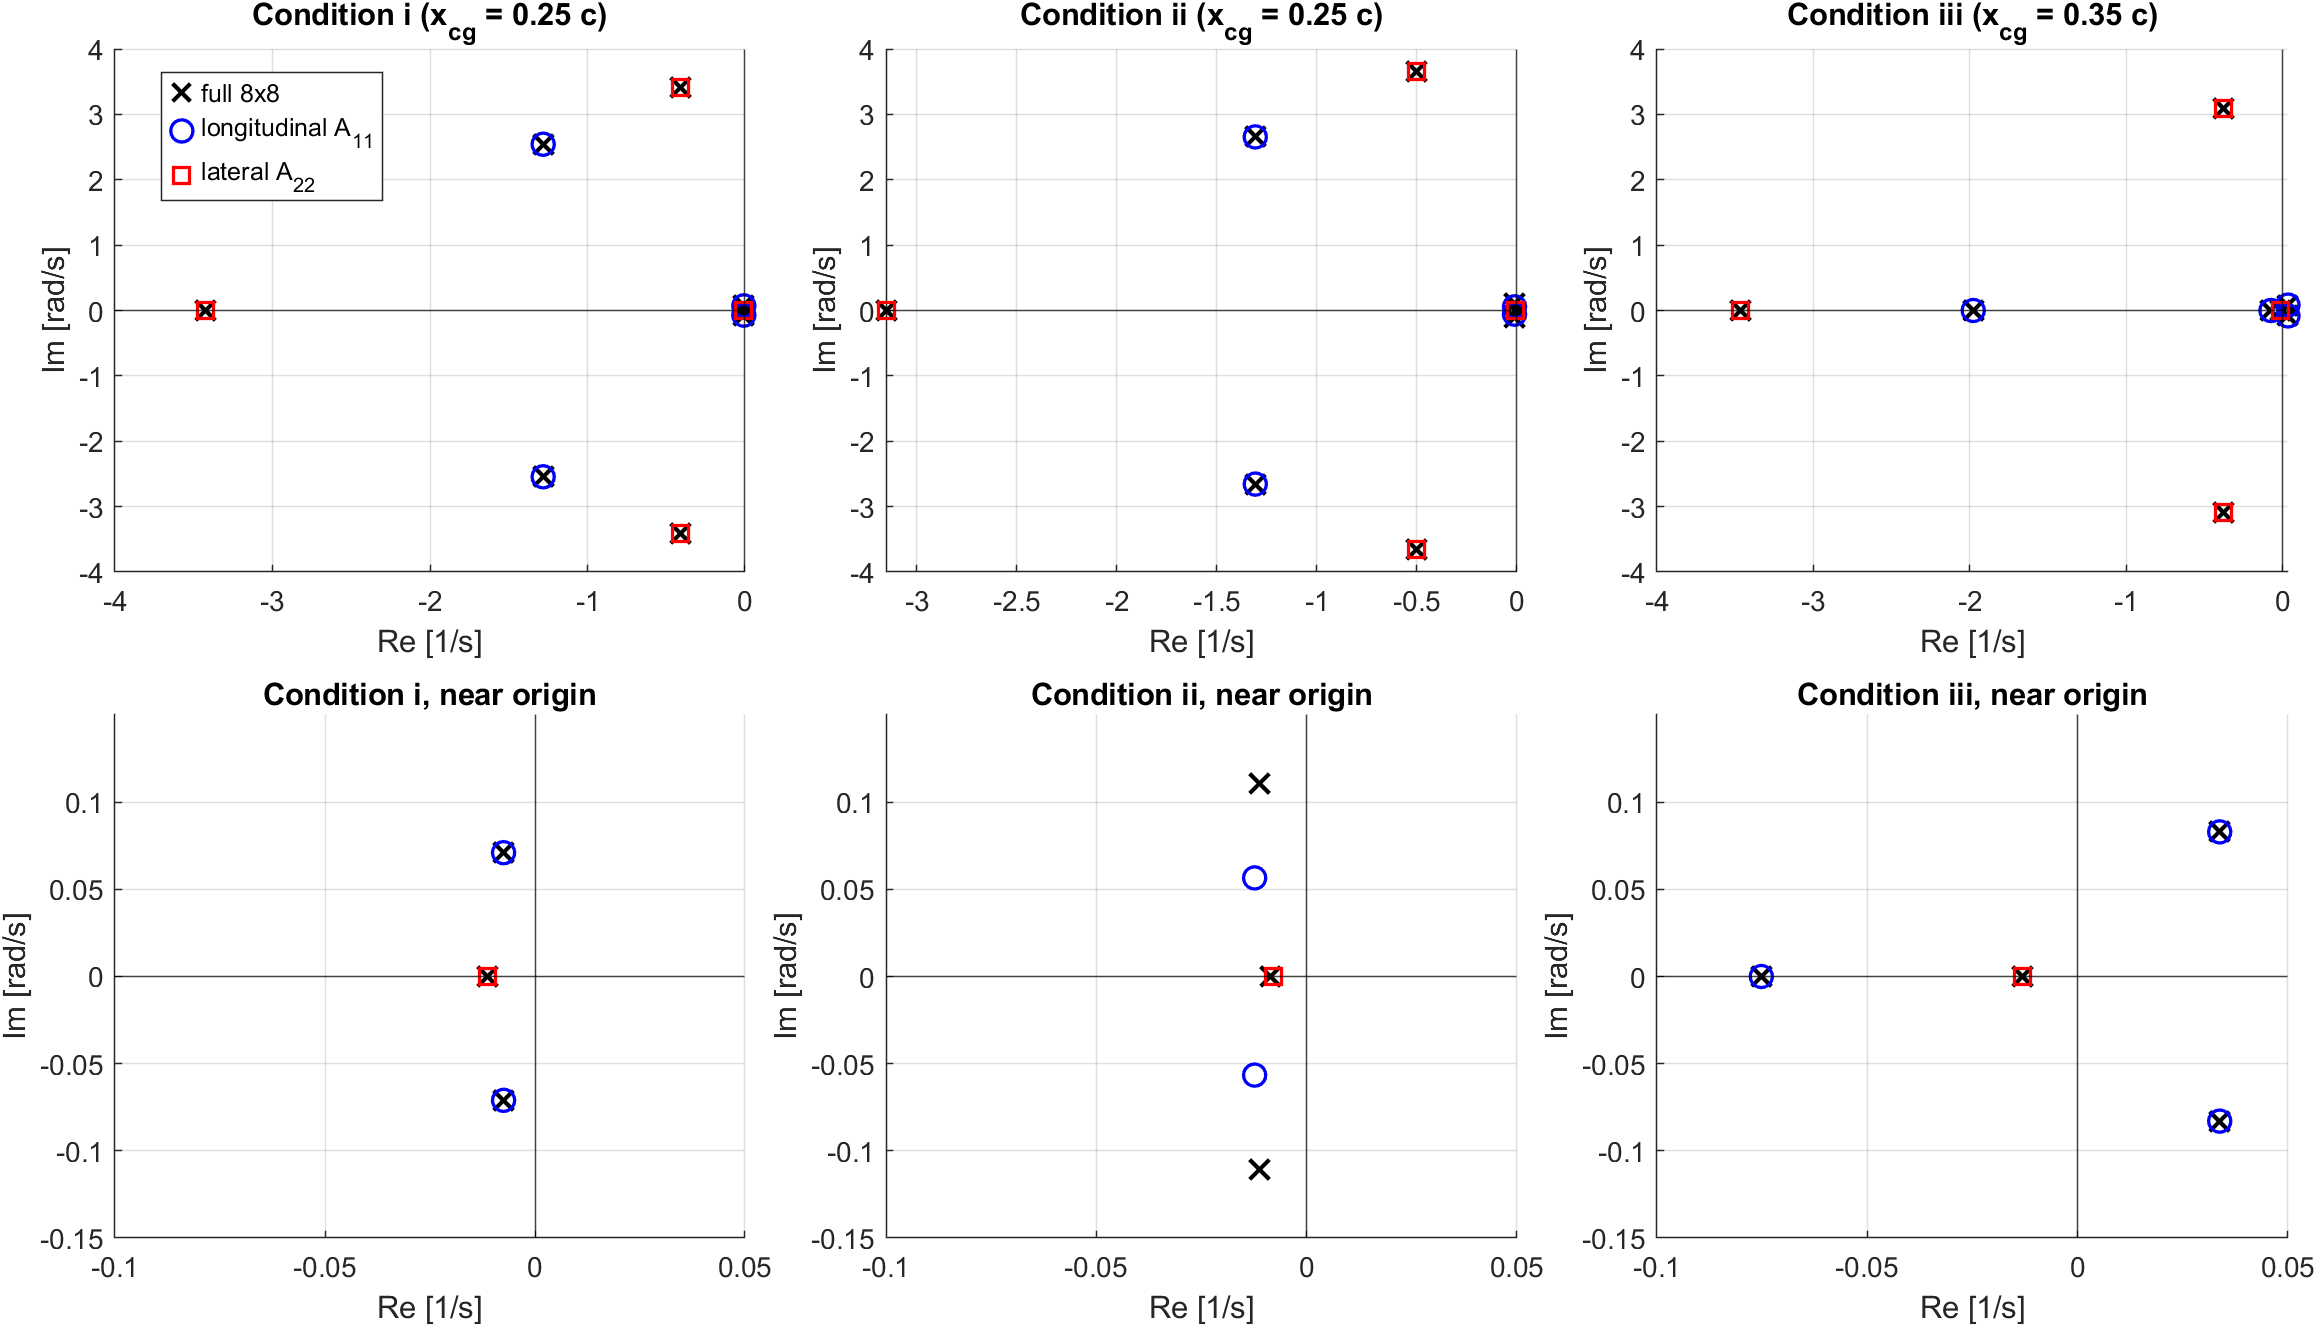
\includegraphics[width=\textwidth]{figures/MT_Eigenvalues.png}
\caption{Eigenvalues of the full model and of the decoupled blocks (top), and the slow modes near the origin (bottom).}
\label{fig:eig}
\end{figure}

\subsection{Comparison of the conditions}
Table~\ref{tab:modes} and Fig.~\ref{fig:eig} give the results. In condition i all modes are stable and classical: a well-damped short period ($\omega_n=2.85$~rad/s, $\zeta=0.45$), a lightly damped phugoid with an 88~s period, a fast roll subsidence ($\tau=0.29$~s), a stable spiral ($t_{1/2}=61$~s) and a lightly damped Dutch roll ($\omega_n=3.44$~rad/s, $\zeta=0.12$). The LEF schedule raises the short-period frequency from 2.53 to 2.85~rad/s (fixed flap: $-1.311\pm2.166j$), because the flap adds pitch stiffness.

Moving the center of gravity to $0.35\bar c$ (condition iii) makes $a_{32}$ positive (Table~\ref{tab:alin}). The short-period pair splits into two real roots: a fast stable root at $-1.978$~s$^{-1}$ and a slow root at $-0.075$~s$^{-1}$. The slow root is close to the phugoid and couples with it, and the phugoid pair moves into the right half-plane, $0.034\pm0.083j$~s$^{-1}$ ($\zeta=-0.38$, $t_2=20.5$~s). This slow oscillatory divergence is what the simulation of Sec.~IV shows. With the flap fixed, the airframe alone has $M_\alpha=+3.47$~s$^{-2}$ and an unstable root at $+0.787$~s$^{-1}$ ($t_2=0.88$~s); the LEF schedule reduces the pitch stiffness to $a_{32}=+1.06$~s$^{-2}$, which is enough to move this root back to the left half-plane, but not to make the aircraft statically stable. The lower directional stability lowers the Dutch-roll frequency to 3.12~rad/s, and the roll and spiral modes change little.

In the turn (condition ii) the fast modes change little from condition i: the short period is slightly stiffer ($\omega_n=2.96$~rad/s), the Dutch-roll damping rises to 0.14 and the roll mode slows to $\tau=0.32$~s. The slow modes change most, because of the coupling discussed below.

For reference, against the MIL-F-8785C limits for a Class IV aircraft in a Category B flight phase~\cite{lec7}, conditions i and ii meet the Level~1 limits for the short-period damping ($0.30\le\zeta\le2$), the phugoid damping ($\zeta>0.04$), the Dutch roll ($\zeta\ge0.08$, $\zeta\omega_n\ge0.15$, $\omega_n\ge0.4$) and the roll time constant ($\tau\le1.4$~s), and have stable spiral modes. The unstable phugoid of condition iii, with $t_2=20.5$~s, does not meet the Level~3 requirement of $T_2\ge55$~s, so condition iii needs the flight control system even with the LEF schedule.

\subsection{Full and decoupled models}
In straight flight (i and iii) the coupling blocks $A_{12}$ and $A_{21}$ are zero, and the modes of the full model and of the decoupled blocks agree to a relative difference of about $10^{-5}$. In the turn, the coupling blocks are not zero: the bank angle enters the vertical force balance ($\partial\dot V_T/\partial\phi=-0.673$, $\partial\dot V_T/\partial\beta=8.56$), and the trim rates link pitch and yaw. The fast modes are almost unaffected (Table~\ref{tab:modesdec}), but the phugoid and spiral modes, whose frequencies are close, interact. In the full model the phugoid period drops from 111~s to 57~s and its damping from 0.21 to 0.10, and the spiral time constant changes from 126~s to 116~s. The eigenvectors confirm the mixing: the longitudinal share is 0.68 for the phugoid pair and 0.48 for the spiral root. Physically, a change of bank in the turn changes the vertical component of the lift and starts a climb or descent with a speed change, and the resulting speed and pitch changes alter the turn. The decoupled blocks therefore misrepresent the slow dynamics in turning flight, and the full model must be used.

\section{Conclusions}
\begin{enumerate}
\item The Homework 1 model, trimmed in Homework 2, holds the trim in wings-level flight and through a complete $60^\circ$ banked turn with fixed controls: deviations stay below $10^{-2}$~m/s and $10^{-3}$~deg, and the turn reproduces the trim turn rate and the theoretical turn radius within 0.2\,\%.
\item The residual motions in the simulations show the dynamic modes: the phugoid and the decaying Dutch roll in condition i, and the coupled phugoid--spiral oscillation in condition ii.
\item With the center of gravity at $0.35\bar c$ the aircraft is statically unstable in pitch ($C_{m_\alpha}=+0.156$~rad$^{-1}$, neutral point near $0.31\bar c$). With the LEF schedule in the linear model, the short period splits into two stable real roots and the phugoid becomes unstable ($t_2=20.5$~s), which matches the slow divergence of the simulation; with the flap fixed, the airframe has an unstable root with $t_2=0.88$~s.
\item All derivatives have their normal signs at the forward center of gravity. $C_{D_u}$ and $C_{m_u}$ vanish in straight flight because the data do not depend on Mach number; the thrust adds a nonzero $X_{T_u}$.
\item In turning flight the elements of $A$ contain inertial and gyroscopic terms in addition to the aerodynamic derivatives, and the slow longitudinal and lateral-directional modes are coupled; the full model is needed there.
\end{enumerate}

\begin{thebibliography}{9}
\bibitem{tp1538} Nguyen, L. T., Ogburn, M. E., Gilbert, W. P., Kibler, K. S., Brown, P. W., and Deal, P. L., ``Simulator Study of Stall/Post-Stall Characteristics of a Fighter Airplane With Relaxed Longitudinal Static Stability,'' NASA TP-1538, 1979.
\bibitem{slj} Stevens, B. L., Lewis, F. L., and Johnson, E. N., \emph{Aircraft Control and Simulation: Dynamics, Controls Design, and Autonomous Systems}, 3rd ed., John Wiley \& Sons, Hoboken, NJ, 2016.
\bibitem{lec5} ``Lecture 5 -- Linearization of Equations of Motion,'' UUM 523E lecture notes, Istanbul Technical University, Fall 2026--2027.
\bibitem{lec6} ``Lecture 6 -- Longitudinal and Lateral-Directional Dynamics,'' UUM 523E lecture notes, Istanbul Technical University, Fall 2026--2027.
\bibitem{lec7} ``Lecture 7 -- Flying and Handling Qualities,'' UUM 523E lecture notes, Istanbul Technical University, Fall 2026--2027.
\end{thebibliography}

\end{document}
